%%%%%%%%%%%%%%%%%%%%%%%%%%%%%%%%%%%%%%%%%%%%%%%%%%%%%%%%%%%%%%%%%%%%%%%%%%%%%%%%
% simulation.tex: Chapter on ECAL Timing
%%%%%%%%%%%%%%%%%%%%%%%%%%%%%%%%%%%%%%%%%%%%%%%%%%%%%%%%%%%%%%%%%%%%%%%%%%%%%%%%
\chapter{Timing Reconstruction and Calibration}
%%%%%%%%%%%%%%%%%%%%%%%%%%%%%%%%%%%%%%%%%%%%%%%%%%%%%%%%%%%%%%%%%%%%%%%%%%%%%%%%
The time of an electromagnetic object such as a photon is extracted at the level of individual crystals called reconstructed hits~(rechits). The recorded time of the photon is the crystal calibrated time where the Time-Of-Flight~(TOF) as well as the time to transmit the recorded signal from the front-end detectors to the back-end readout electronics is removed such that on average the time is zero for a photon produced at the nominal proton-proton collision point and travelling at speed of light and then impinges at the surface of the crystal.  There are separate algorithms for extracting and calibrating the crystals using the rechit time. This calibrated time is considered the reconstructed time~($T_{RECO}$). 
Measuring the difference in timing between any two reconstructed objects ( individual crystals or electromagnetic objects) originating from the same nominal point and thus assumed in principle to have the same time give the timing resolution of the detector as well as the crystal-to-crystal synchronization factor.  $T_{RECO}$ of a photon can be defined in either of the following ways:
\begin{enumerate}
\item Seed Time: The time of the highest energy crystal or rechit in the highest energy basic cluster of the photon supercluster denoted as $T_{SEED}$
\item The Mean Time: This is the error weighted mean time of all the crystals in the photon supercluster denoted as $T_{CLUSTER}$ or $T_{MEAN}$ and is defined as follows:
\begin{equation}
T_{CLUSTER} = T_{MEAN} = \frac{\sum_{i=1}^N\frac{T_{i}}{\sigma_{i}^{2}}}{\sum_{i=1}^{N}\frac{1}{\sigma_{i}^{2}}} 
\end{equation}
\newline
 where N is the number of crystals in seed basic cluster of photon supercluster. 

\end{enumerate}
\subsection{Electromagnetic Calorimeter Readout Chain}
%%%%%%%%%%%%%%%%%%%%%%%%%%%%%%%%%%%%%%%%%%%%%%%%%%%%%%%
The ECAL electronics readout system described in detailed in \cite{ECALREADOUT} is a light-to-light system. Energy from incoming electromagnetic objects is absorbed and converted into scintillating light by \pb crystals. This is received and converted into electrical signals by the avalanche photo-diodes. These electrical signals are digitized and finally converted back into light signals which is transported using optical fibres into the off detector electronics in the counting room at point 5. Thus one can easily classify the full readout chain of the ECAL electronics readout system as divided into an on-detector electronics and an off-detector electronics.
Both electronics system are connected by a 100~m optical fibre links. A simple picture of the readout chain is shown in fig{FIXME:Fig readout Chain}.

%%%%%%%%%%%%%%%%%%%%%%%%%%%%%%%%%%%%%%%%%%
The on-detector electronics reads a trigger tower consisting of $5\times5$ crystals in $\eta \times \phi$ in barrel~(EB) and \textit{supercrystals} in endcap~(EE). Five Very Front End~(VFE) boards (reading out data from 5 crystals each), one Front End boad~(FE) two~(EB) and six~(EE) Giga Optical Hybrids~(GOH), one Low Voltage Regulator~(LVR) board and a Mother Board~(MB) make up the complete on-detector electronics. Electrical Signals from the APDs~(EB) are accepted by the VFE which is equipped with a Multi Gain Pre-Amplifier~(MGPA), a 12-bit Analogue to Digital Converter~(ADC) and a buffer. The MGPA an Application Specific Intergrated Circuit~(ASIC) developed in 0.25~$\mu$m technology, pre-amplifiers, shapes and then amplifies the signals through three amplifiers with gains of 1, 6 and 12. For VPT~(EE), these signals first pass through a High Voltage~(HV)filter card which acts as a moderator separating very high voltages caused by the increase radiation in the EE. The full scale of the APDs and VPTs are 60~pC and 12.8~pC corresponding to $\approx$ 1.5~TeV and 1.6-3.1~ TeV respectively. The full shaping of the signal takes about 40~ns. The noise for gain 12 is about 8000$e^{-}$ for APD configuration and about 4000$e^{-}$ for VPT configuration. 
The 3 analog output signals of the MPGA are digitized in parallel by the multichannel 40~MHz, 12-bit ADC. This ADCs have an effective number of bits of 10.9. The highest non-saturated signal is selected as the output signal and reported as 12 bits of the corresponding ADC with 2 bits coding the ADC number. It is possible, that when the signal is saturated and wrong signal amplitude can be produced leading to am amplitude dependence of the readout time. This effect has been studied for Gain 1 and 6 transitions and the relevant corrections factors of timing produced and validated.
A schematics picture of the showing the readout chain of the FE with its MPGA and ADCs showing the shaping and digitization process can be seen in figure \eqref{readout}.

\begin{center}\label{readout}
\centering
\mbox{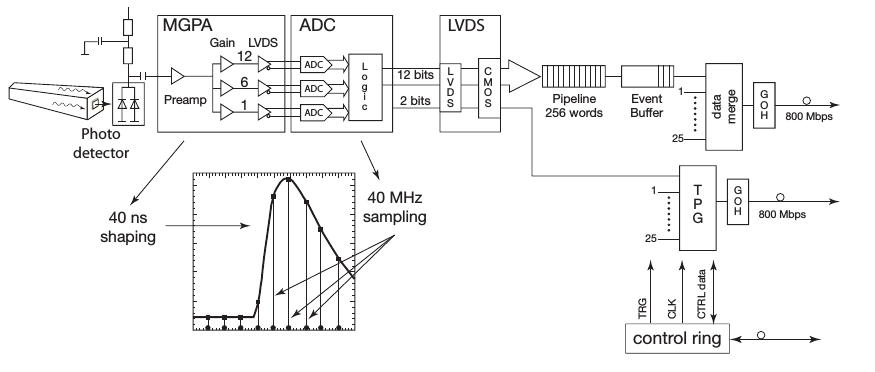
\includegraphics[scale=0.6]{/home/tensr/Documents/TEN-HEP-PHD-THESIS/PHD_THESIS/PHD/THESISPLOTS/ReadOut.png}} 
\captionof{figure}{Schematic showing ReadOut Chain.}
\label{fig:readout}
\end{center}

A radiation-hard buffer~(LVDS) adapts a low voltage differential out put signal of the ADC to input into the FE. Signals from  five  identical channels are integrated and read into VFE card with a Detector Control Unit for measuring  the APD leakage currents. The noise from each VFE is typically 1.1, 0.75, 0.6 ADC counts for gains 12, 6 and 1 respectively. This would be about 40~MeV for gain 12.

Digitized data from 5 VFE cards are fed into each FE through the LVDS and stored in 256-word-deep dual-ported memories called pipelines. Data pipelines can be stored for up to 128 bunch crossings. The FE is base on a ASIC called the FERNIX holding the logic to calculated the energy of 5 channels once every bunch crossing. This energy is summed in strips of 5 crystals  along $\phi$. Thus each VFE is serviced by a FERNIX chip. In the case of the EE, the five strip energy sum are transported by GOH to the off-detector electronics Trigger Concentration Card~(TCC) while for EB, there a sixth FERNIX which sums the five strips energy sums  and calculates an electromagnetic bit which is used to identify electromagnetic shower candidates on the basis of their shower profile in a trigger tower. The trigger tower energy sums and the electromagnetic bit is transmitted to the TCC through the GOH. This process is referred to as Trigger Primitive Genration~(TPG). Once a Level-1 trigger signal is received, the ten 40~MHz samples for each channel are transmitted to the off-detector electronics DCC using an identical GOH. This takes about 7.5~$\mu$s. The VFE and FE cards are controlled using a 40~MHz digital optical link system and controlled by the off-detector Clock and Control System~(CCS). 
The Off-detector electronics consist of different types of electronic boards~(the CCS, TCC and DCC modules) sitting in an 18 VME-9U crates and a 1 VME-6U crate holding the Selective Read-Out Processor~(SRP). This system is serving both the trigger and the  Data Acquisition Systems~(DAQ) paths. In the DAQ path, the DCC performs data read-out and data reduction based on flags of the SRP. While in the trigger path, at each bunch crossing, the trigger primitive generation which began in the FE is finalised and synchronised or time alignments in the TCC before transmitted to the regional calorimeter triggers. The trigger primitives each refer to a single trigger tower~(25 crystal data) and consists of  the summed transverse energy deposits and the electromagnetic bit charactering the lateral shower profile of the electromagnetic shower. The accept signal for accepted events is return from the global trigger after about 3~$\mu$sand the selected events area read into the data acquisition system to the filter farm where the even rate is further reduced using data from the full detector. Thus is the regional calorimeter, the ECAL trigger primitives  together with the HCAL trigger primitives are used to  compute the electron/photon and jet candidates as well as their transverse energy. The resulting physics objects after passing through the HLT trigger are transferred to the various tier systems for offline full event reconstruction. The ECAL also has a laser calibration systems where laser light is delivered directly to the \pb crystals using optical fibres. The laser data is used for energy and time calibration of crystals and hardware system. The crystals are energy calibrated because of the decrease in optical transmission due to the formation of color centres in the crystal. The formation of color centres is caused by irradiation. Time calibration using laser data is also required in case of hardware timing offset especially during long short down periods of the CMS detectors.
 %%%%%%%%%%%%%%%%%%%%%%%%%%%%%%%%%%%%%%%%%%%%%%%%%%%%%%%%%%%%%%%%%%%%%%%%%%%%%%%%
\subsection{Timing Extraction}
%%%%%%%%%%%%%%%%%%%%%%%%%%%%%%%%%%%%%%%%%%%%%%%%%%%%%%%%%%%%%%%%
The MGPA of the VFE amplifies and shapes an analogue signal from the APD/VPT of a single crystal producing a typical signal pulse as seen in figure \eqref{pulse}. 

\begin{center}\label{pulse}
\centering
\mbox{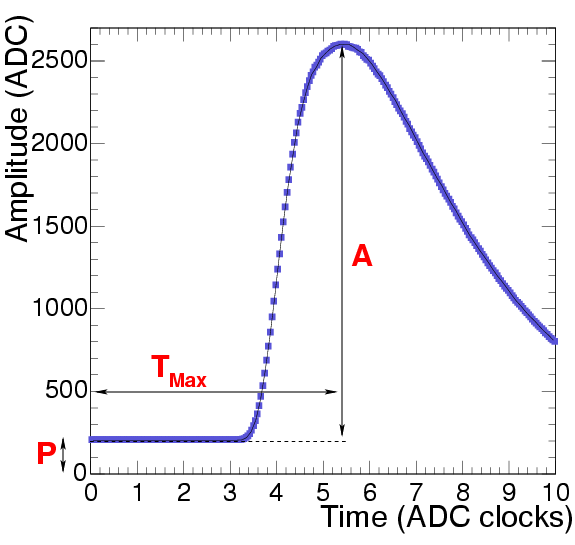
\includegraphics[scale=0.6]{THESISPLOTS/Time_Amplitude_Profile.png}}
%\mbox{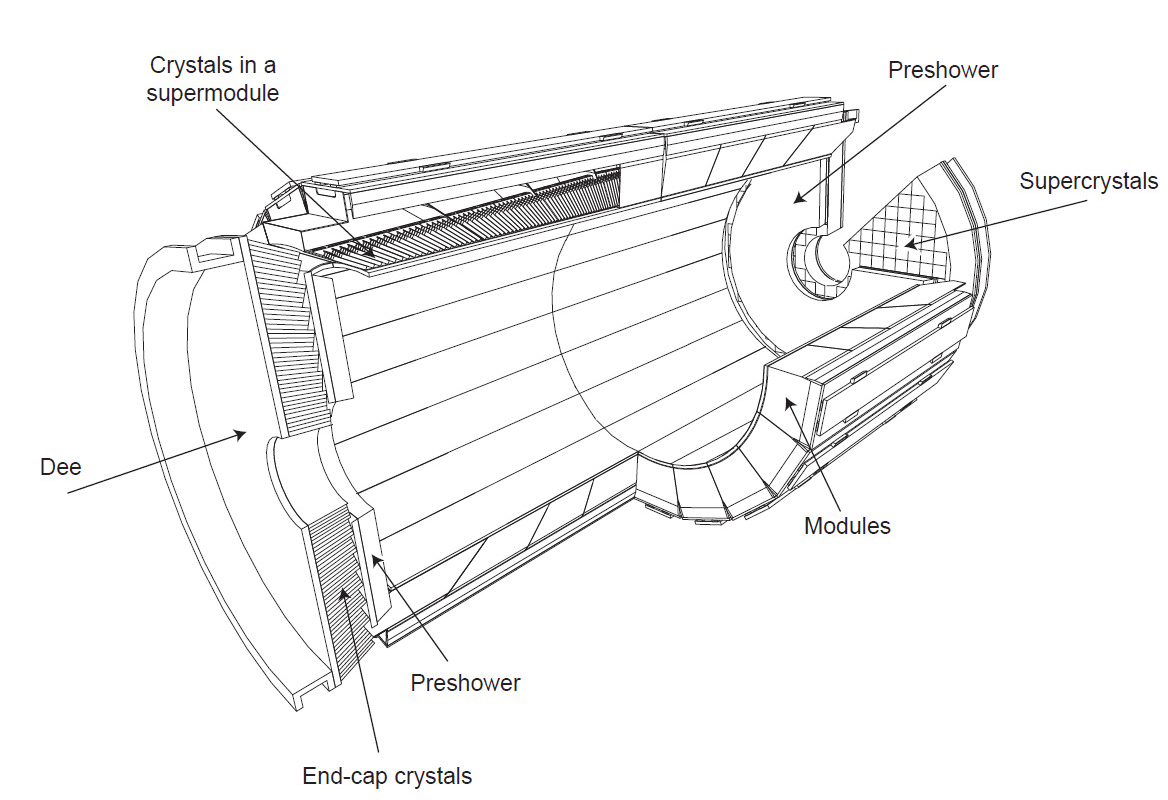
\includegraphics[scale=0.2]{THESISPLOTS/CMS-ECAL.png}}
%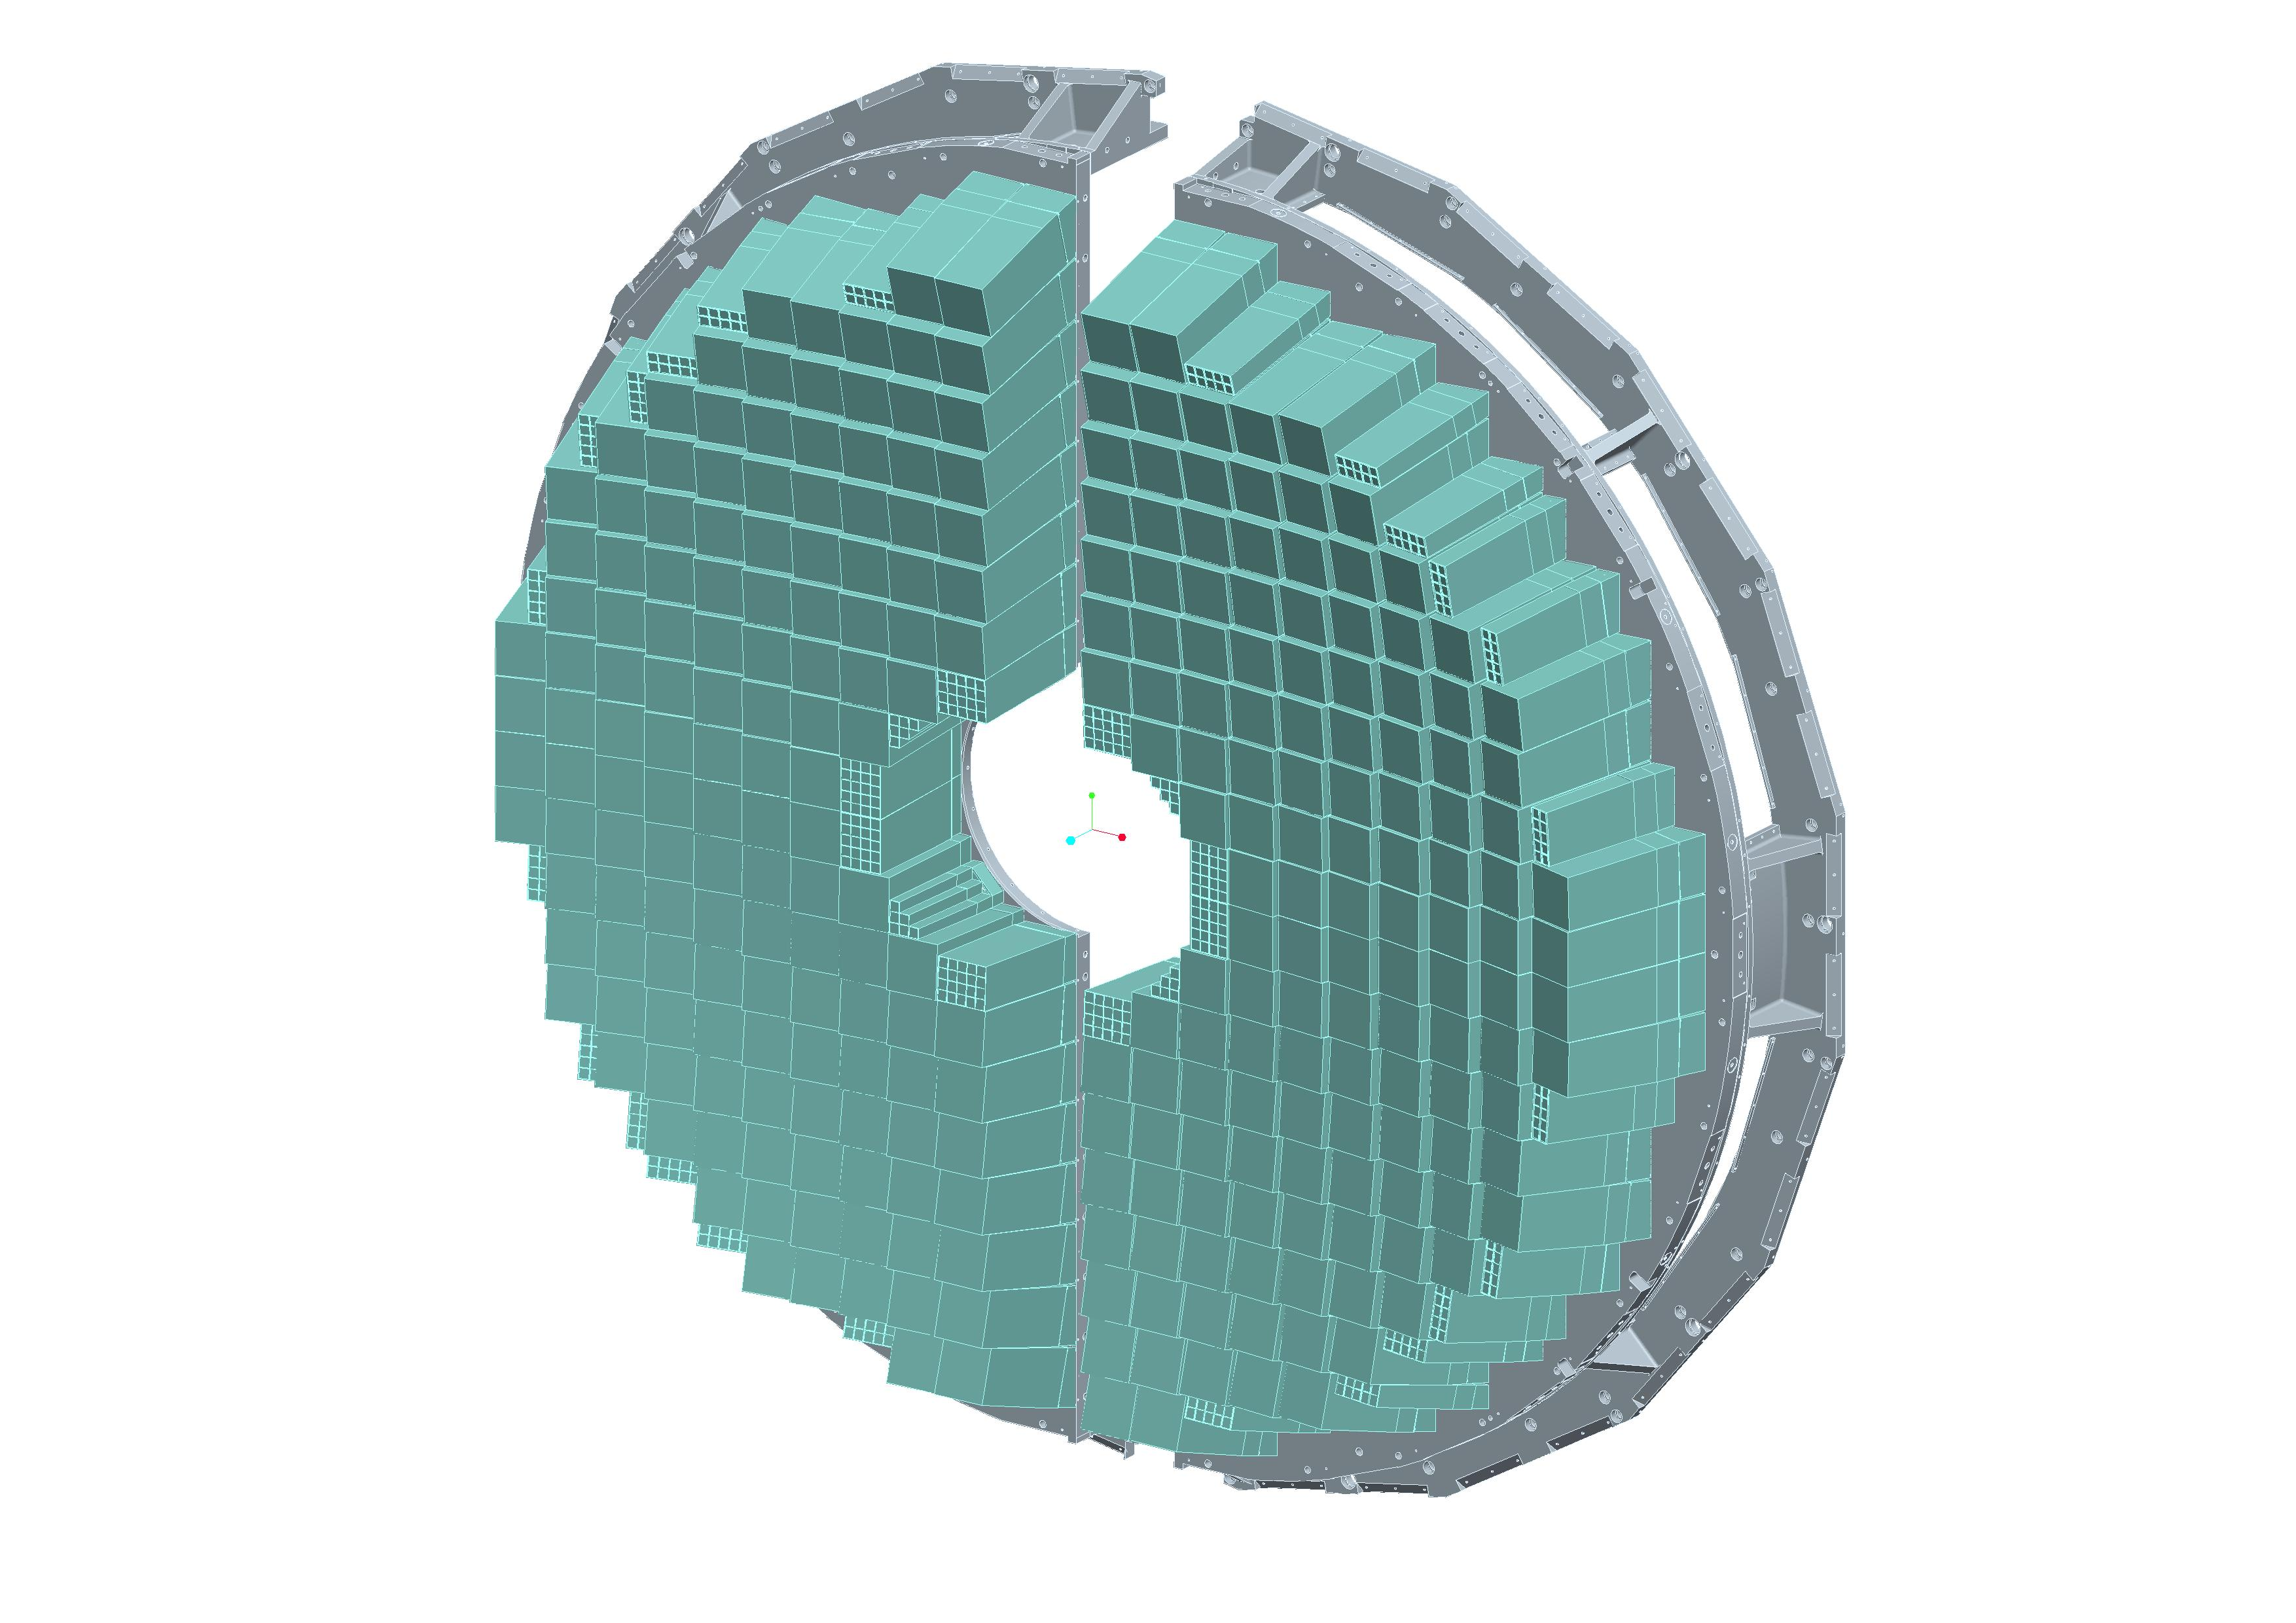
\includegraphics[scale=0.06]{THESISPLOTS/endcap_CMS.png}} 
\captionof{figure}{Typical pulse shape of a given signal showing signal amplitude and time.}
\label{fig:pulse}
\end{center}

This pulse is digitised into 10 samples by the ADC for data storage purposes. The pulse's amplitude  is a measure of the energy deposited in the crystal while the time from the ADC clock with a sampling frequency of 40~MHz for 10 samples is used to extract the arrival time of the physics object depositing its energy unto the crystal. The value \textbf{P} is known as the pedestal or noise read as ADC values in the absence of any signal. Using the 10 samples, a timing algorithm is employed to extract the time of arrival of particles to the ECAL. The goal of this algorithm is to use the maximum amplitude value of the pulse $A_{MAX}$, and extract its corresponding maximum value of the ADC time $A_{MAX}$ as the time of arrival of the physics object to the crystal. Thus, ECAL timing reconstruction is defined as: Using the 10 samples of the pulse amplitude to measure $T_{MAX}$. Obtaining the true $A_{MAX}$ is performed through an energy reconstruction algorithm. Extracting the arrival time is thus a matter of comparing the pulse shape obtained using the 10 samples of a scintillating channel's pulse to that of a reference shape.
This reference shape is obtained from experimental measurements using Testbeam or synchronous LHC events. Figure \label{amplVsTmax}(a) shows a distribution of the amplitude $A$ as a function of time rather plotted for convenience as $A/A_{MAX}$ on the vertical or $y$-axis and $T - T_{MAX}$ on the horizontal or $x$-axis. $T$ is the time and $T_{MAX}$ is defined as the time when the  pulse reaches its maximum value, $A_{MAX}$ 

\begin{center}\label{amplVsTmax}
\centering
\mbox{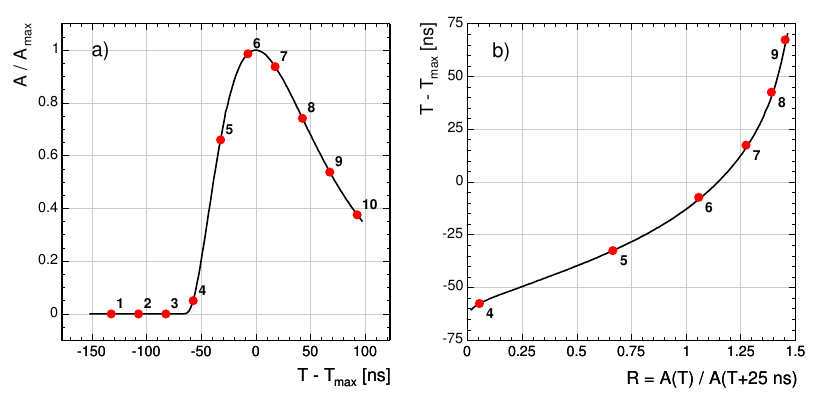
\includegraphics[scale=0.45]{THESISPLOTS/AmplitudeVsTMax.png}} \quad
\mbox{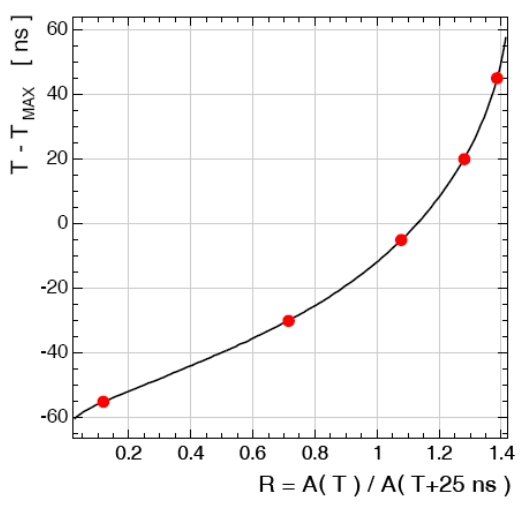
\includegraphics[scale=0.45]{THESISPLOTS/TMaxPhaseVsRatio.png}}
%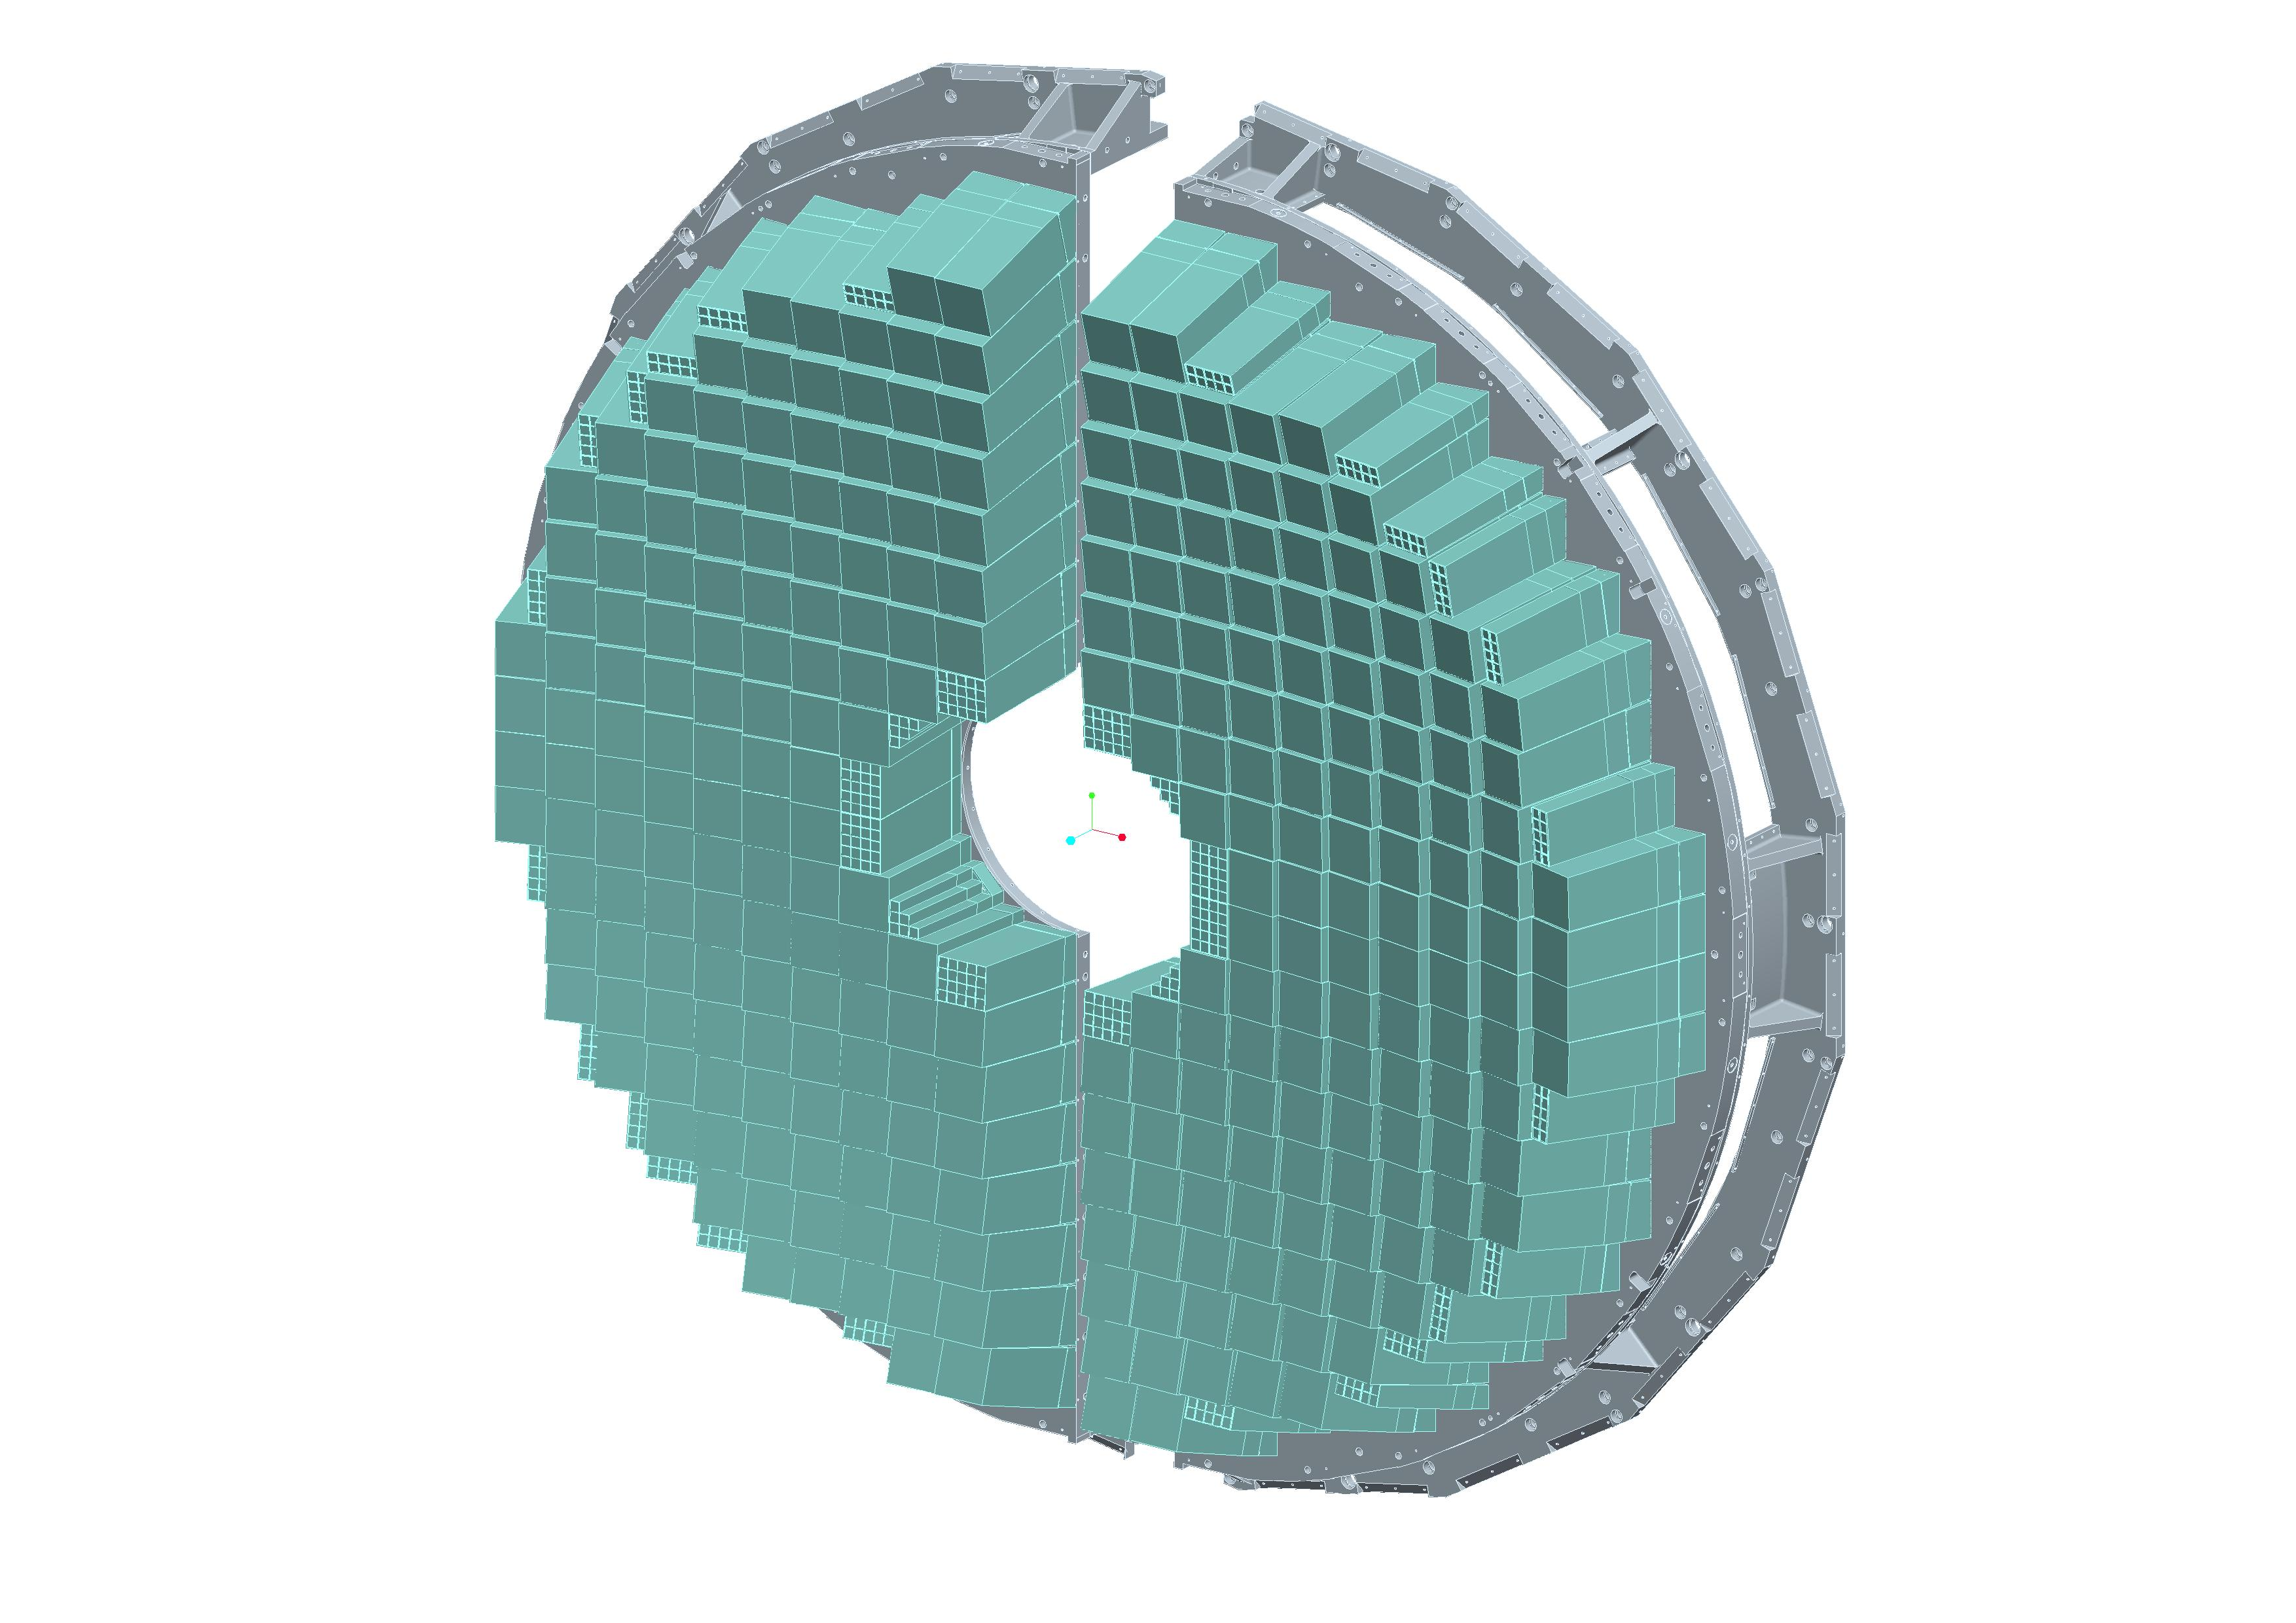
\includegraphics[scale=0.06]{THESISPLOTS/endcap_CMS.png}} 
\captionof{figure}{left: A measured ECAL pulse shape for each channel. Right: $T - T_{MAX}$ Vs $ R(T)$ showing the distribution of $T(R)$. Solid line is reference shape or shape from testbeam while dots correspond to a 10 discrete samples corresponding to signal from a single event in a single channel or crystal. }
\label{fig:amplVsTmax}
\end{center}

Performing an analytical fit to compare the reference pulse shape to that from the 10 samples on the $A(T)$ distribution to obtain $A_{MAX}$ and $T_{MAX}$ is rather cumbersome and technically in efficient, as the amplitude of each sample depends on the pulse shape, the $A_{MAX}$ value and also the relative position of $T_{MAX}$ between time samples. This phase is referred to as "\textit{$T_{MAX}$ phase}".
Thus, using a new variable defined as $R(T) = A(T)/ A(T + 25~\mbox{ns})$ and instead perform an analytical fit on the distribution of $T - T_{MAX}$ Vs $ R(T)$. This  $T(R)$ distribution is independent on $A_{MAX}$ and can be very well described by a polynomial of order 7. A distribution of $T(R)$ is shown in figure \eqref{amplVsTmax}(b) with both the four to five samples(dots) obtained from the ratio $R_{i} = A_{i}/A_{i+1}$ from each consecutive pair of samples and the reference pulse shape(continuous line). Thus each point $R_{i}$ gives a quick accurate measurement of $T_{MAX,i} = T_{i} - T(R_{i})$. The uncertainty, $\sigma_{T,i}$, on each measurement is a production of the derivative of the function $T(R)$ and the uncertainty on the value of $R_{i}$. The uncertainty on the value of $R_{i}$ depends on three separate uncertainties: the noise fluctuation, $\sigma_{n}$ of each sample, the uncertainty in the estimation of the pedestal value which is always subtracted from the measured value and the truncation during 12-bit digitization. These uncertainties are uncorrelated and can thus be added in quadrature.
The reconstructed time and its error of a hit(fraction of energy deposited on a single crystal) is determine using the following equations:


\begin{equation}
\displaystyle{T_{MAX} = \frac{\sum \frac{T_{MAX,i}}{\sigma^{2}_{i}}}{\sum \frac{1}{\sigma^{2}_{i}}}} \quad ; \quad\quad
\displaystyle{\frac{1}{\sigma^{2}_{T}} =  \sum \frac{1}{\sigma^{2}_{i}} }
\end{equation}

where the sum is over all the 4 or 5 $R_{i}$ ratios and the assumption is that the weights are uncorrelated. 

%%%%%%%%%%%%%%%%%%%%%%%%%%%%%%%%%%%%%%%%%%%%%%%%%%%%%%%%%%%
\subsection{Timing Resolution}
%%%%%%%%%%%%%%%%%%%%%%%%%%%%%%%%%%%%%%%%%%%%%%%%%%%%%%%%%%%
Using the reconstructed timing for each channel, We can measure the timing resolution for ECAL.
First, the timing resolution for ECAL can be parametrised and expressed as a sum in quadrature ~(uncorrelated) of three major terms accounting for the uncertainties in the timing measurement. These three contributions are: First, the noise~($N$) resulting from contributions from electronic noise, coherent movement of the baseline and effects due to the fact that in addition to the main or hard proton-proton collision, other soft or less energetic collisions or events are produced known as \textit{pile up}~(PU) effect. Second, the stochastic term~($S$) resulting from fluctuations in the photon collection time because of finite time for \pb scintillation. Finally the constant term~($C$) whose contribution is independent on the energy deposited but rather from effects correlated with the point of shower initiation within the crystal and systematics in the extraction of the time due to different is pulse shape for each channel.
The equation for the timing resolution can thus be expressed as shown in equation \eqref{TimeRes}

\begin{equation}\label{TimeRes}
\sigma^{2}(t) = \left(\frac{N\sigma_{n}}{A}\right)^{2} + \left(\frac{S}{\sqrt{A}}\right)^{2} + C^{2}
\end{equation}
$A$ is the measured amplitude corresponding to the energy deposited and $\sigma_{n}$ is the intrinsic noise for individual sample with a value of $\approx 42$~MeV and $140$~MeV in the barrel and endcap respectively and $N = 33$~ns measured from Monte carlo simulation studies. Contribution from the stochastic term, ($S$) is considered small, with value of $S < 7.9$~ns$\cdot MeV^{1/2}$.
\newline
To measure the timing resolution, a simple experiment was performed in which electron beams with energies between $15$~GeV(GeV = Giga electron volts = $10^{6}$~eV, 1~eV$ = 1.602 \times 10^{-19}$~joules~(J) in energy units) and $250$~GeV was directed unto each crystal in a supermodule. The timing resolution measurement is obtained by extracting from the measured distribution of the difference in timing between two crystals sharing energy from the same electromagnetic shower. The advantage of this approach is that, the contribution from poor synchronisation is less as this synchronisation effects do not affect the spread but rather the average time. However, it is not blind to crystal-to-crystal synchronisation effects.
Other methods used to study timing resolution is considering the timing difference between two a few group of crystals usually $5\times5$  crystals called basic clusters, between a complete electromagnetic shower or electron or photon.

Using equation \eqref{TimeRes} and neglecting the stochastic term because its contributions are negligible, the timing resolution can be expressed as:
 
 \begin{equation}\label{ResTime}
 \sigma^{2}(t_{1} - t_{2}) = \left(\frac{N\sigma_{n}}{A_{eff}}\right)^{2} + 2\bar{C}^{2}
 \end{equation}
 
 where $A_{eff} = A_{1}A_{2}/\sqrt{A^{2}_{1} + A^{2}_{2}}$, $t_{1,2}$ and $A_{1,2}$ correspond to the times and amplitude measured in the two crystals and $\bar{C}$ is their residual contribution.
Measuring the timing resolution is performed by using the standard deviation of the Gaussian fit of the distribution from each slice in $A_{eff}/\sigma_{n}$ distribution. The $\sigma(t_{1} - t_{2})$ against $A_{eff}/\sigma_{n}$ of the extracted standard deviation of each slice is plotted the resulting distribution fitted to extract the noise and constant term. The results are shown in figure \eqref{FitTimeRes} with the noise factor $N = (35.1 \pm 0.2)$~ns and $\bar{C} = (20 \pm 4)$ ~ns. 

\begin{center}\label{fittimeRes}
\centering
\mbox{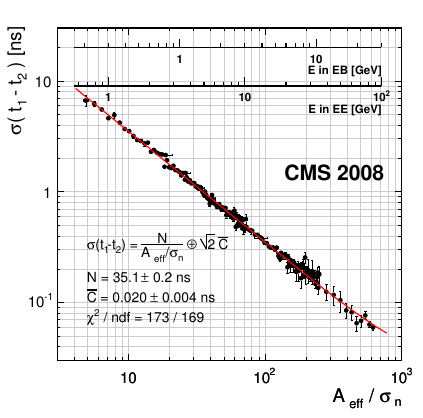
\includegraphics[scale=0.8]{THESISPLOTS/ECAL_Timing_Resolution.png}}
%\mbox{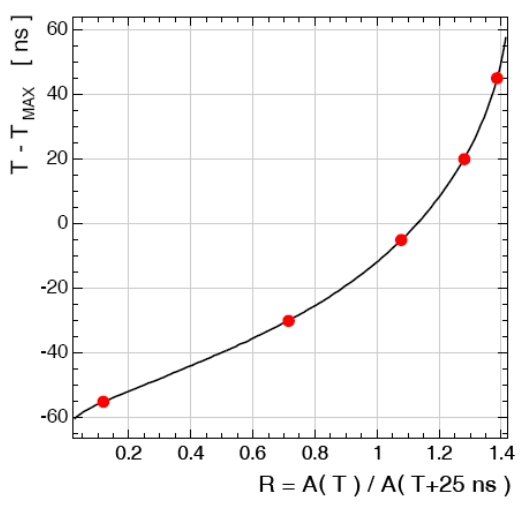
\includegraphics[scale=0.45]{THESISPLOTS/TMaxPhaseVsRatio.png}}
%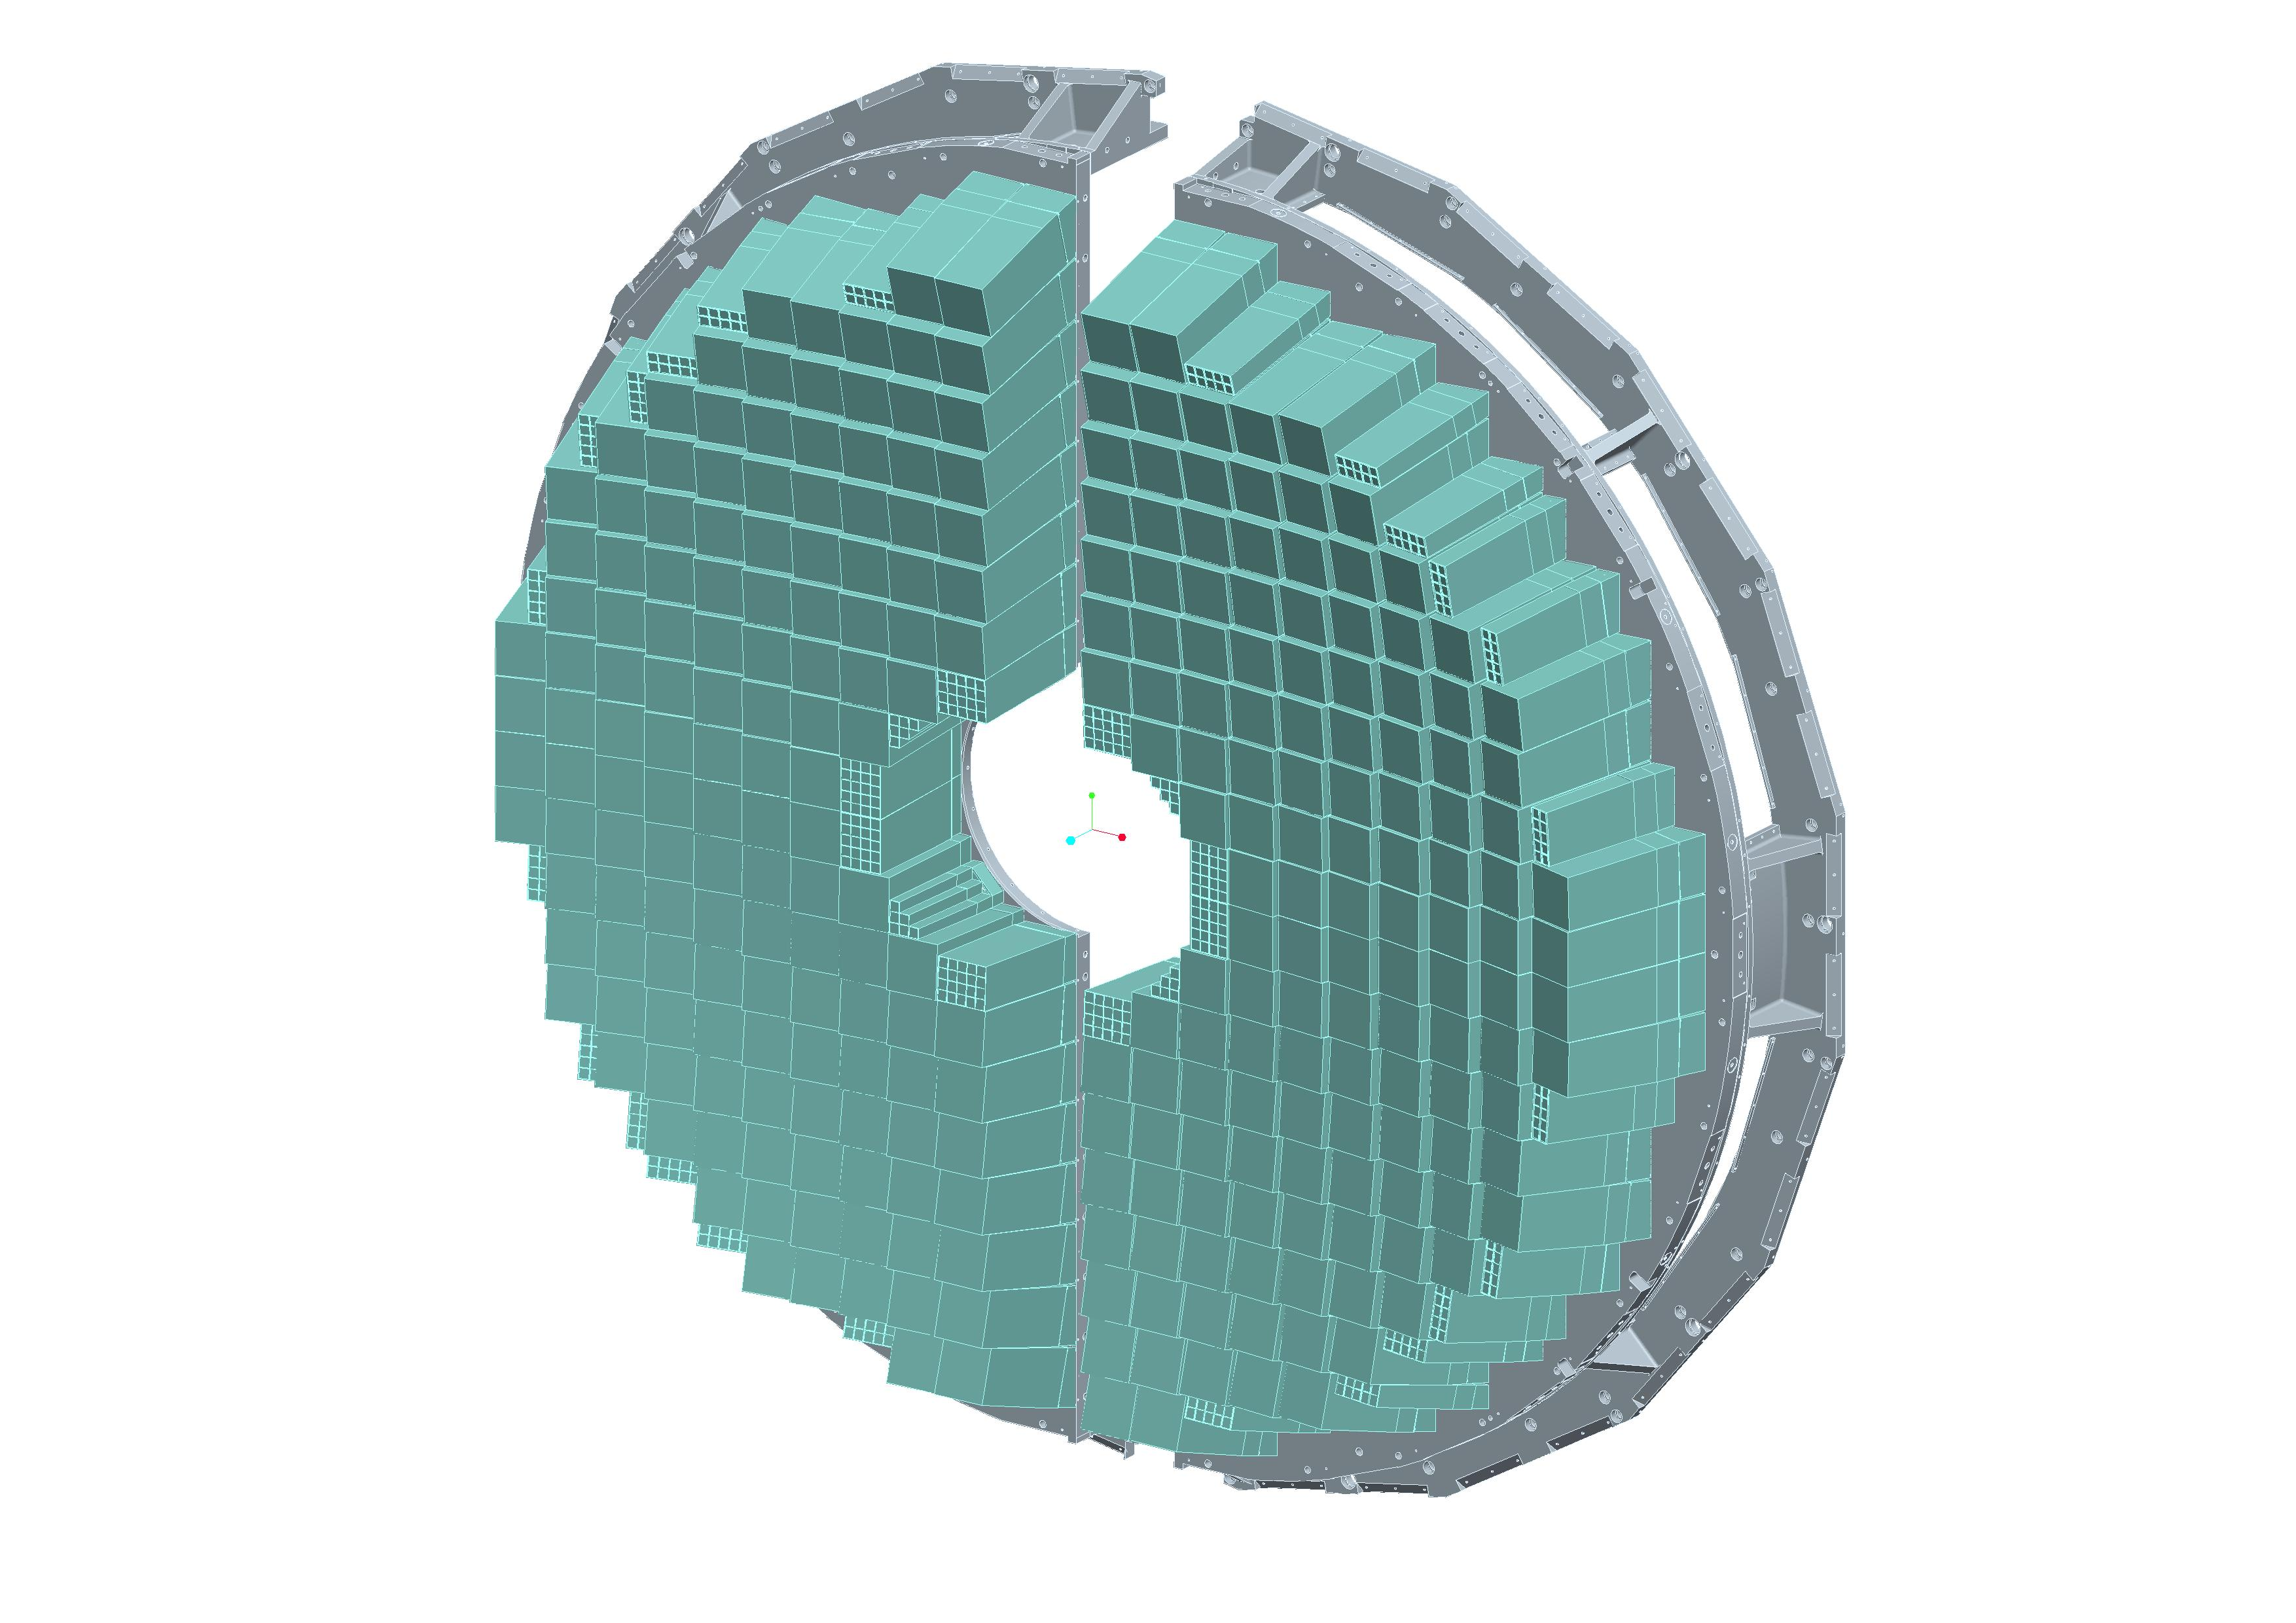
\includegraphics[scale=0.06]{THESISPLOTS/endcap_CMS.png}} 
\captionof{figure}{Deviation of the timing difference as a function of $A_{eff}/\sigma_{n}$ between two crystals sharing an energy in the same electromagnetic shower obtained during electron testbeam measurements. The single crystal energy scales for barrel~(EB) and endcap~(EE) is overlaid. The fitted results give $N = (35.1 \pm 0.2)$~ns and $\bar{C} = (20 \pm 4)$ ~ns. }
\label{fig:FitTimeRes}
\end{center}
A timing resolution better than $100$~ps for energy values $A_{eff}/\sigma_{n}$ greater than $400$~ADC counts is obtained. This demonstrates that for a perfectly calibrated ECAL crystals and energy deposits of $E > 20$~GeV in the barrel, we can obtain a resolution better than $100$~ps. 

%%%%%%%%%%%%%%%%%%%%%%%%%%%%%%%%%%%%%%%%%%%%%%%%%
\subsection{Timing Calibration Procedure}
%%%%%%%%%%%%%%%%%%%%%%%%%%%%%%%%%%%%%%%%%%%%%%%%%%%%%
The timing calibration is performed such that particles travelling along a straight path with speed close to the speed of light or $\beta \approx 1$ produced from proton-proton collisions happening at the CMS luminous region or IP will arrive at the surface of an ECAL crystal  with an average time of 0~ns. This means that if a particle arrives at a crystal with its arrival time significantly and positively large, then it is either because this particle is travelling with a very small velocity (slowly moving particles or  $\beta << 1$ ) or it was produced with a decay path that  significantly deviates from the obvious straight path connecting the arrived at crystal to the IP or it is a particle from the decay of a temporarily stopped particle in the detector.
The presence of the "$T_{MAX}$ Phase", the difference in pulse shape between each crystal, variation in time of flight by a few nanosecond~(ns) and the different intrinsic delays among channels allow for timing calibration at two separate levels.
At the level of the front end electronics ~(FE) consisting of $5\times5$ crystals, one is capable of performing an initial internal timing synchronization by adjusting in steps of 1.04~ns among these crystals. Determining these values of adjustments to be made is referred to as \textit{Hardware Synchronization}.

\subsubsection{Offline Timing Calibration}
%%%%%%%%%%%%%%%%%%%%%%%%%%%%%%%%%%%%%%%%%%%%%%%%%%%%%%%%%%%%%%%%%%
The purpose of the offline calibration is to provide additive timing adjustments values for each channel measured from reconstructed data to account for global phase shift in timing caused by shifts in CMS clock relative to the LHC bunch crossings and de-synchronizations induced by hardware interventions occurring usually during detector repairs. The global shifts due to drifting in CMS clock relative to LHC bunch crossings can be about 1~ns while that caused by hardware intervention can be about 3~ns. The calibration constants obtained for each crystal or channel are the negative values of the average time measured from the reconstructed hits of each crystals.
These crystals are  kept in XML files which are then loaded into the online configuration database holding the hardware settings. The calibration procedure is as follows:first identify the existence of a timing shift occurrence using either the CMS or ECAL detector running electronic~(e-Log) book or the CMS or ECAL data acquisition monitoring~(DQM) results. Second, if there is a timing shift, use reconstructed crystals hits or rechits from very recently produced data to measure the calibration constants for each channel. Finally deploy the validated calibration constants in an XML format file into the online configuration database for reprocessing of CMS full datasets to be used for physics analysis.
This process is repeated over and over until the entire LHC proton-proton collision period each year. At the end of each calibration process, the set of calibration constants developed for the hardware settings within a period of time is referred to as having an \textit{interval of validity or IOVs}. The amount of data used in measuring the timing constants is defined by the amount of event statistics available and covers a particular CMS events run range. During the entire LHC run period of 2011, a total of 17 IOVs were developed while during 2012 LHC run, a total of 44 IOVs were produced. The raw dataset used in producing the calibration constants are mostly ECAL crystals hits from Level-1 triggered events with loosely triggered electromagnetic objects including a photons, electrons and hadrons with larger electromagnetic proportions called \textit{ElectronHad} or \textit{PhotonHad}. These event rechits must pass the following selection criteria: The event time~(an average over its rechits) must be smaller than 5~ns. Event rechits must belong to a basic cluster~(cluster of about $5\times5$ crystals) with transverse energy of atleast 2~GeV. The signal amplitude must not be lower than 26(47) or 100~(in year 2012) ADC counts for rechits in EB(EE)   corresponding to an energy of about 1(3)~GeV respectively. The reconstructed rechit time must be within 5(7)~ns window in EB(EE) respectively and to reduce the presence of anomalous crystal hits, the ratio of the sum of energies of the north, south, east and west neighbouring crystals excluding a crystal with the highest energy to that of the energy of the highest energy crystal must be greater than 5\%  or equivalently $ 1 - E_{4}/E_{1} < 0.95$. This variable is known as the \textit{swiss-cross} variable and it is very useful for rejecting events with anomalous crystal energy deposits. The selected rechits are used to make a timing distribution for each channel and if each channel has at least 10 rechits, the average time measured represents the timing calibration constants or inter-calibration coefficient to be applied for correction while the spread or variance represents the spread in this measurement. For channels with less than 10 valid rechits, the average time of all the other channels is assigned to them as their inter-calibration coefficient. validation of these constants is obtained by applying the negative value of these constants to the same or a different set of events and varying that the measured average over rechits per channel is 0~ns to within the accuracy of the calibration method and event migration in the event sample. The event migration effects are of the order of 10~ps.
The figures in figure \ref{fig:TimeCalib} shows a two dimensional distribution of the channel mean time for each crystal for all the 61,200 crystals in the EB and 1468 crystals in EE. Its shows the mean timing distribution prior to calibration and after the measured calibration constants have been applied.
The full IOVs produced for the entire LHC runs 2011 and 2012 can be found here \cite{ECALTIMECALIB}.
%%%%%%%%%%%%%%%%%%%%%%%%%%%%%%%%%%%%%%%%%%%%%%%%%%%%%%%%%%%%%%%%%
\begin{center}\label{TimeCalib}
\centering
\mbox{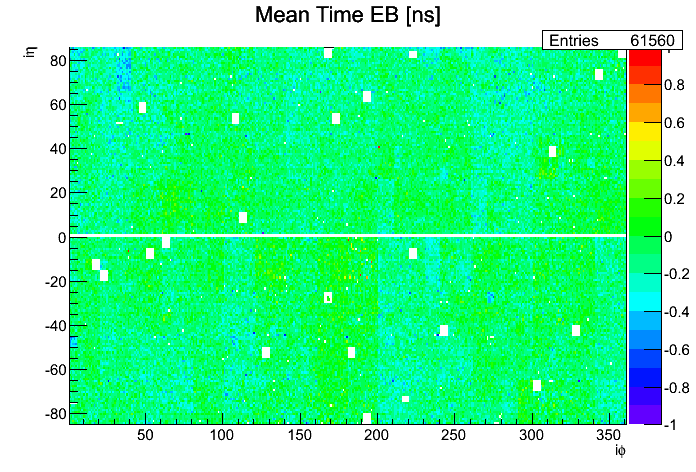
\includegraphics[scale=0.35]{THESISPLOTS/calibDiffMapEB_Before_Calibration.png}}
\mbox{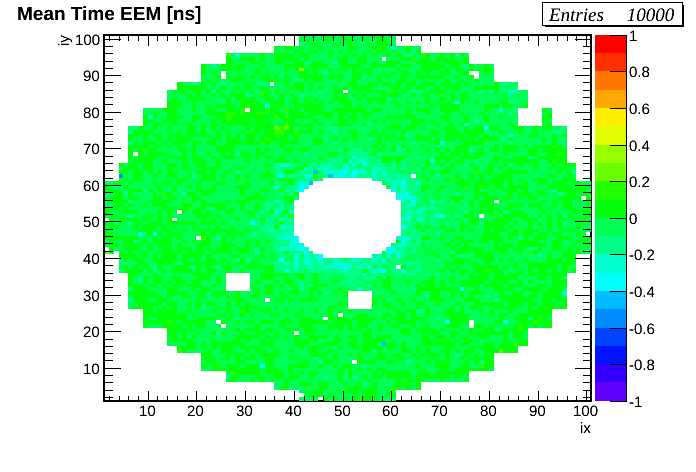
\includegraphics[scale=0.28]{THESISPLOTS/calibDiffMapEEM_Before_CALIB.png} \quad
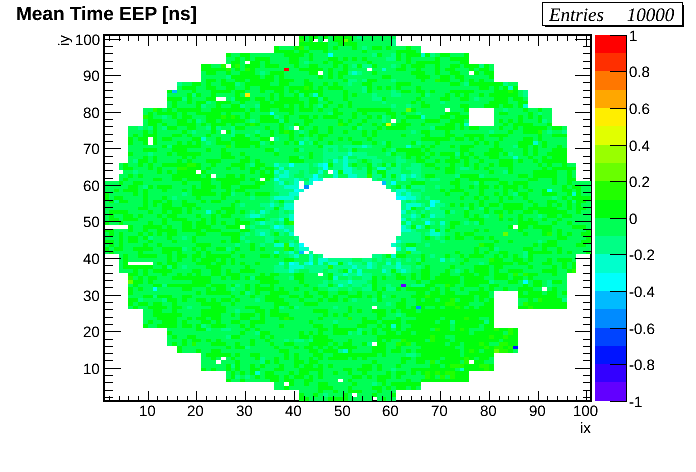
\includegraphics[scale=0.28]{THESISPLOTS/calibDiffMapEEP_Before_CALIB.png}
}
\vspace{3cm}

\mbox{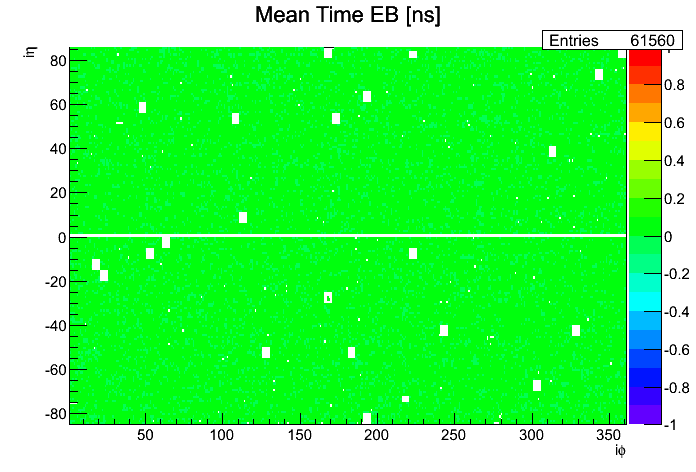
\includegraphics[scale=0.35]{THESISPLOTS/calibDiffMapEB_After_Calibration.png}}
\mbox{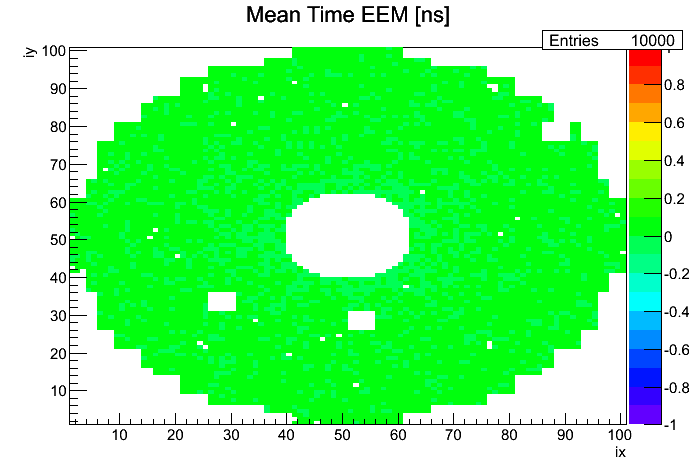
\includegraphics[scale=0.28]{THESISPLOTS/calibDiffMapEEM_AFter_CALIB.png} \quad
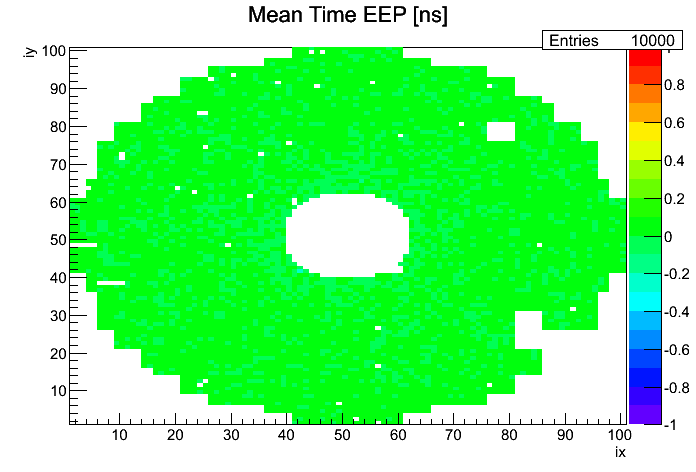
\includegraphics[scale=0.28]{THESISPLOTS/calibDiffMapEEP_After_CALIB.png}
}
\captionof{figure}{Top: Timing calibration maps showing the distribution of average time for each channel/\pb crystal in EB~(top) and EE~(below: EE\texttt{-}(left), EE\texttt{+}(right)) before calibration.\newline
Bottom: Timing calibration maps showing the distribution of average time for each channel/\pb crystal in EB~(top) and EE~(below: EE\texttt{-}(left), EE\texttt{+}(right)) after calibration. 
After calibration most crystals have an average time of zero.}
\label{fig:TimeCalib}
\end{center}

\subsubsection{Hardware Timing Calibration}
%%%%%%%%%%%%%%%%%%%%%%%%%%%%%%%%%%%%%%%%%%%%%%%%%%%%%%%%%%%%%%%%%%%
Often, it happens that during a regular technical stop or machine development period, the hardware experts maintaining the ECAL front end electronics introduce a timing offset due to hardware intervention. These timing offsets are not easily adjusted at the event reconstruction level, offline, using software from proton-proton collisions data. These hardware settings for readout electronics with timing offsets if not properly aligned can contribute to the worsening of the timing resolution. The traditional method of correcting for this hardware timing latency during CMS data taking when the LHC is colliding protons at stable beams has been to collect enough data with the unadjusted hardware settings with timing offset during stable proton beams, stop the entire CMS data taking process while LHC proton collisions are ongoing and use the collected data to extract the hardware timing offset and finally use these extracted timing offsets to adjust the hardware settings for future collisions when CMS detector data taking has resumed. These offsets are extracted from Data Quality Monitoring~(DQM) and data certification hardware readout electronics performance histograms. However, although these procedure is quite effective, it is not very efficient as stopping the ECAL section of the CMS detector in order to adjust the settings of the hardware readout electronics requires a huge loss in data taking by the entire CMS detector. Since the goal of the CMS data taking department is to minimised the lost of data as much as possible thus reducing the difference between LHC delivered luminosity and CMS recorded luminosity, an efficient approach is needed. We have developed such an approach to investigate and adjust the hardware settings in case of a timing offset at the readout electronics after each period of technical stop or machine development.
Rather than using collision data, we use the laser data whose initial primary objective is to adjust for crystal energy resolution due to loss of crystals transparency through radiation. 
We use laser data to measure hardware timing offset and use these timing offsets provide new hardware settings prior to proton-proton collision. These adjustment is performed at the level of ECAL online readout electronics condition data base. The full procedure for this process can be found at \cite{LaserTiming}. The ECAL laser system comprise of two lasers, a 440~nm wavelength~( close to peak emission for \pb crystals) laser for monitoring crystal transparency lose and a 796~nm wavelength laser for monitoring readout electronics chain from APDs to ADCs. Both lasers have jitter of less than 4~ns for every 24 hours run. To account for this jittering effect, the timing from the laser is averaged over 600 event pulses. The time for each crystal from laser is expected to be the same as the time from data and is represented as $T^{APD}_{MAX} $. The ECAL laser system is also equipped with a fast acquisition card called MATACQ. The time for each channel recorded using the Matacq is also averaged over 600 event pulse denoted as $ T_{Matacq}$.
The difference in $ T^{APD}_{MAX} - T_{Matacq} $ between these two times averaged over a clock and control unit ~(CCU) comprising of 25 crystals gives the time for each CCU denoted as $ t_{CCU} = \left\langle T^{APD}_{MAX} - T_{Matacq} \right\rangle $ average over 25 crystals.
Thus to calculate the timing shift of 25 crystals belonging to the same front end electronics~(FE), we monitor for any changes to the this average before~($t^{B}_{CCU} $) and after~($t^{A}_{CCU} $) hardware intervention.  This difference $\Delta t_{CCU} = t^{A}_{CCU} - t^{B}_{CCU} $ after corrections due to global shift in the average timing~($\left\langle t^{A}_{CCU} - t^{B}_{CCU} \right\rangle $) for all the CCUs in an entire supermodule~(SM) or front end detector~(FED) or single readout unit from the data acquisition point of view. These global timing shift of all the crystals in a given FED is due to the laser light distribution inhomogeneity or evolution of the laser pulse due to different optical fibre supply of laser light to each CCU. Each FED or SM is made of 1,700 \pb crystals. 
The plots in figure \ref{fig:TimeLaser} show our current observation of  monitoring for any shift in timing within each CCU using laser. It shows the distribution of the CCU timing difference $ \Delta t_{CCU}$ with its root mean squared~(RMS) value for each CCU before and after machine intervention. Considering the subtraction of the global shift per FED also reduces the possibility of false timing shift showing up by a given CCU.

\begin{center}\label{TimeLaser}
\centering
\mbox{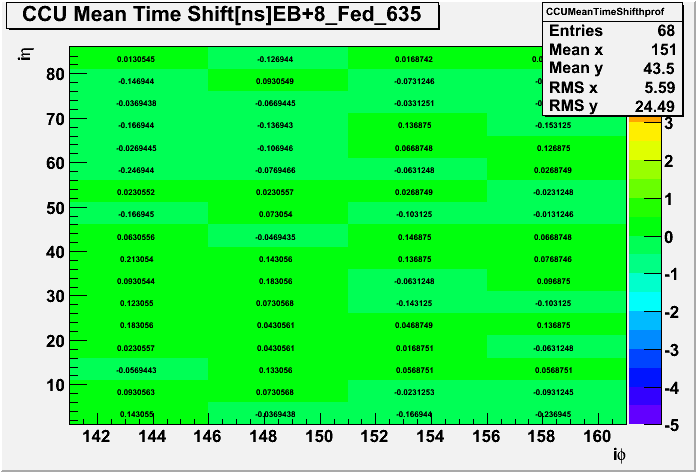
\includegraphics[scale=0.2]{THESISPLOTS/CCU_Mean_Time_ShiftEB_Plus8_Fed_635.png} \quad
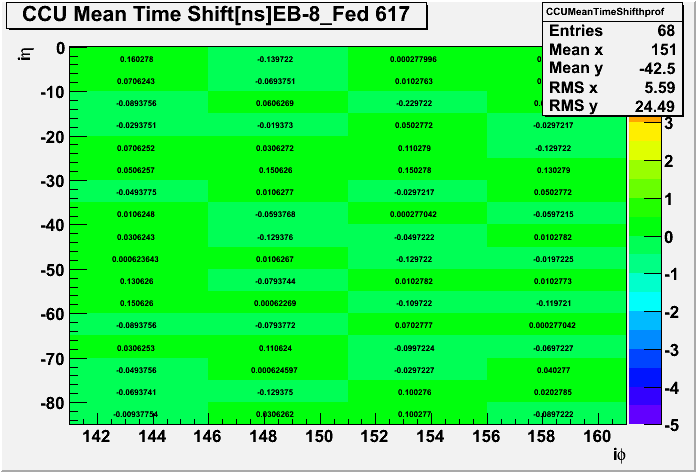
\includegraphics[scale=0.2]{THESISPLOTS/CCU-Mean-Time-Shift-EBMinus8-Fed617.png}}

\vspace{1cm}
\mbox{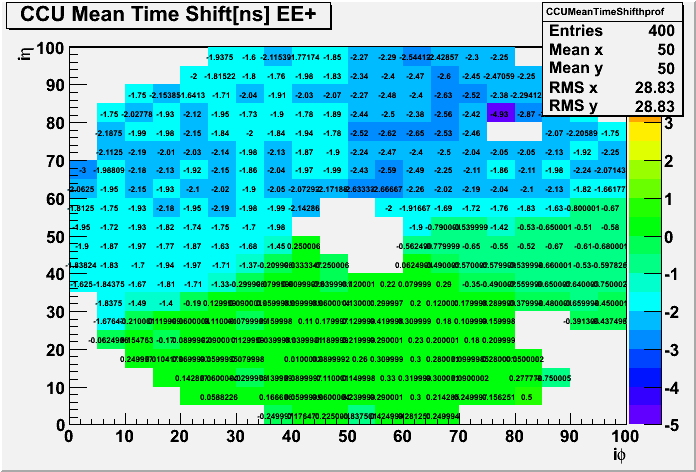
\includegraphics[scale=0.2]{THESISPLOTS/CCU_Mean_Time_Shift_EEP_Laser.png} \quad 
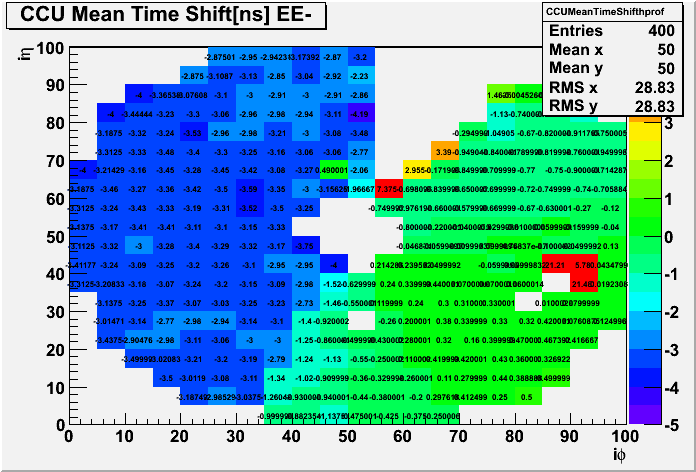
\includegraphics[scale=0.2]{THESISPLOTS/CCU_Mean_Time_Shift_EEM_Laser.png}}
%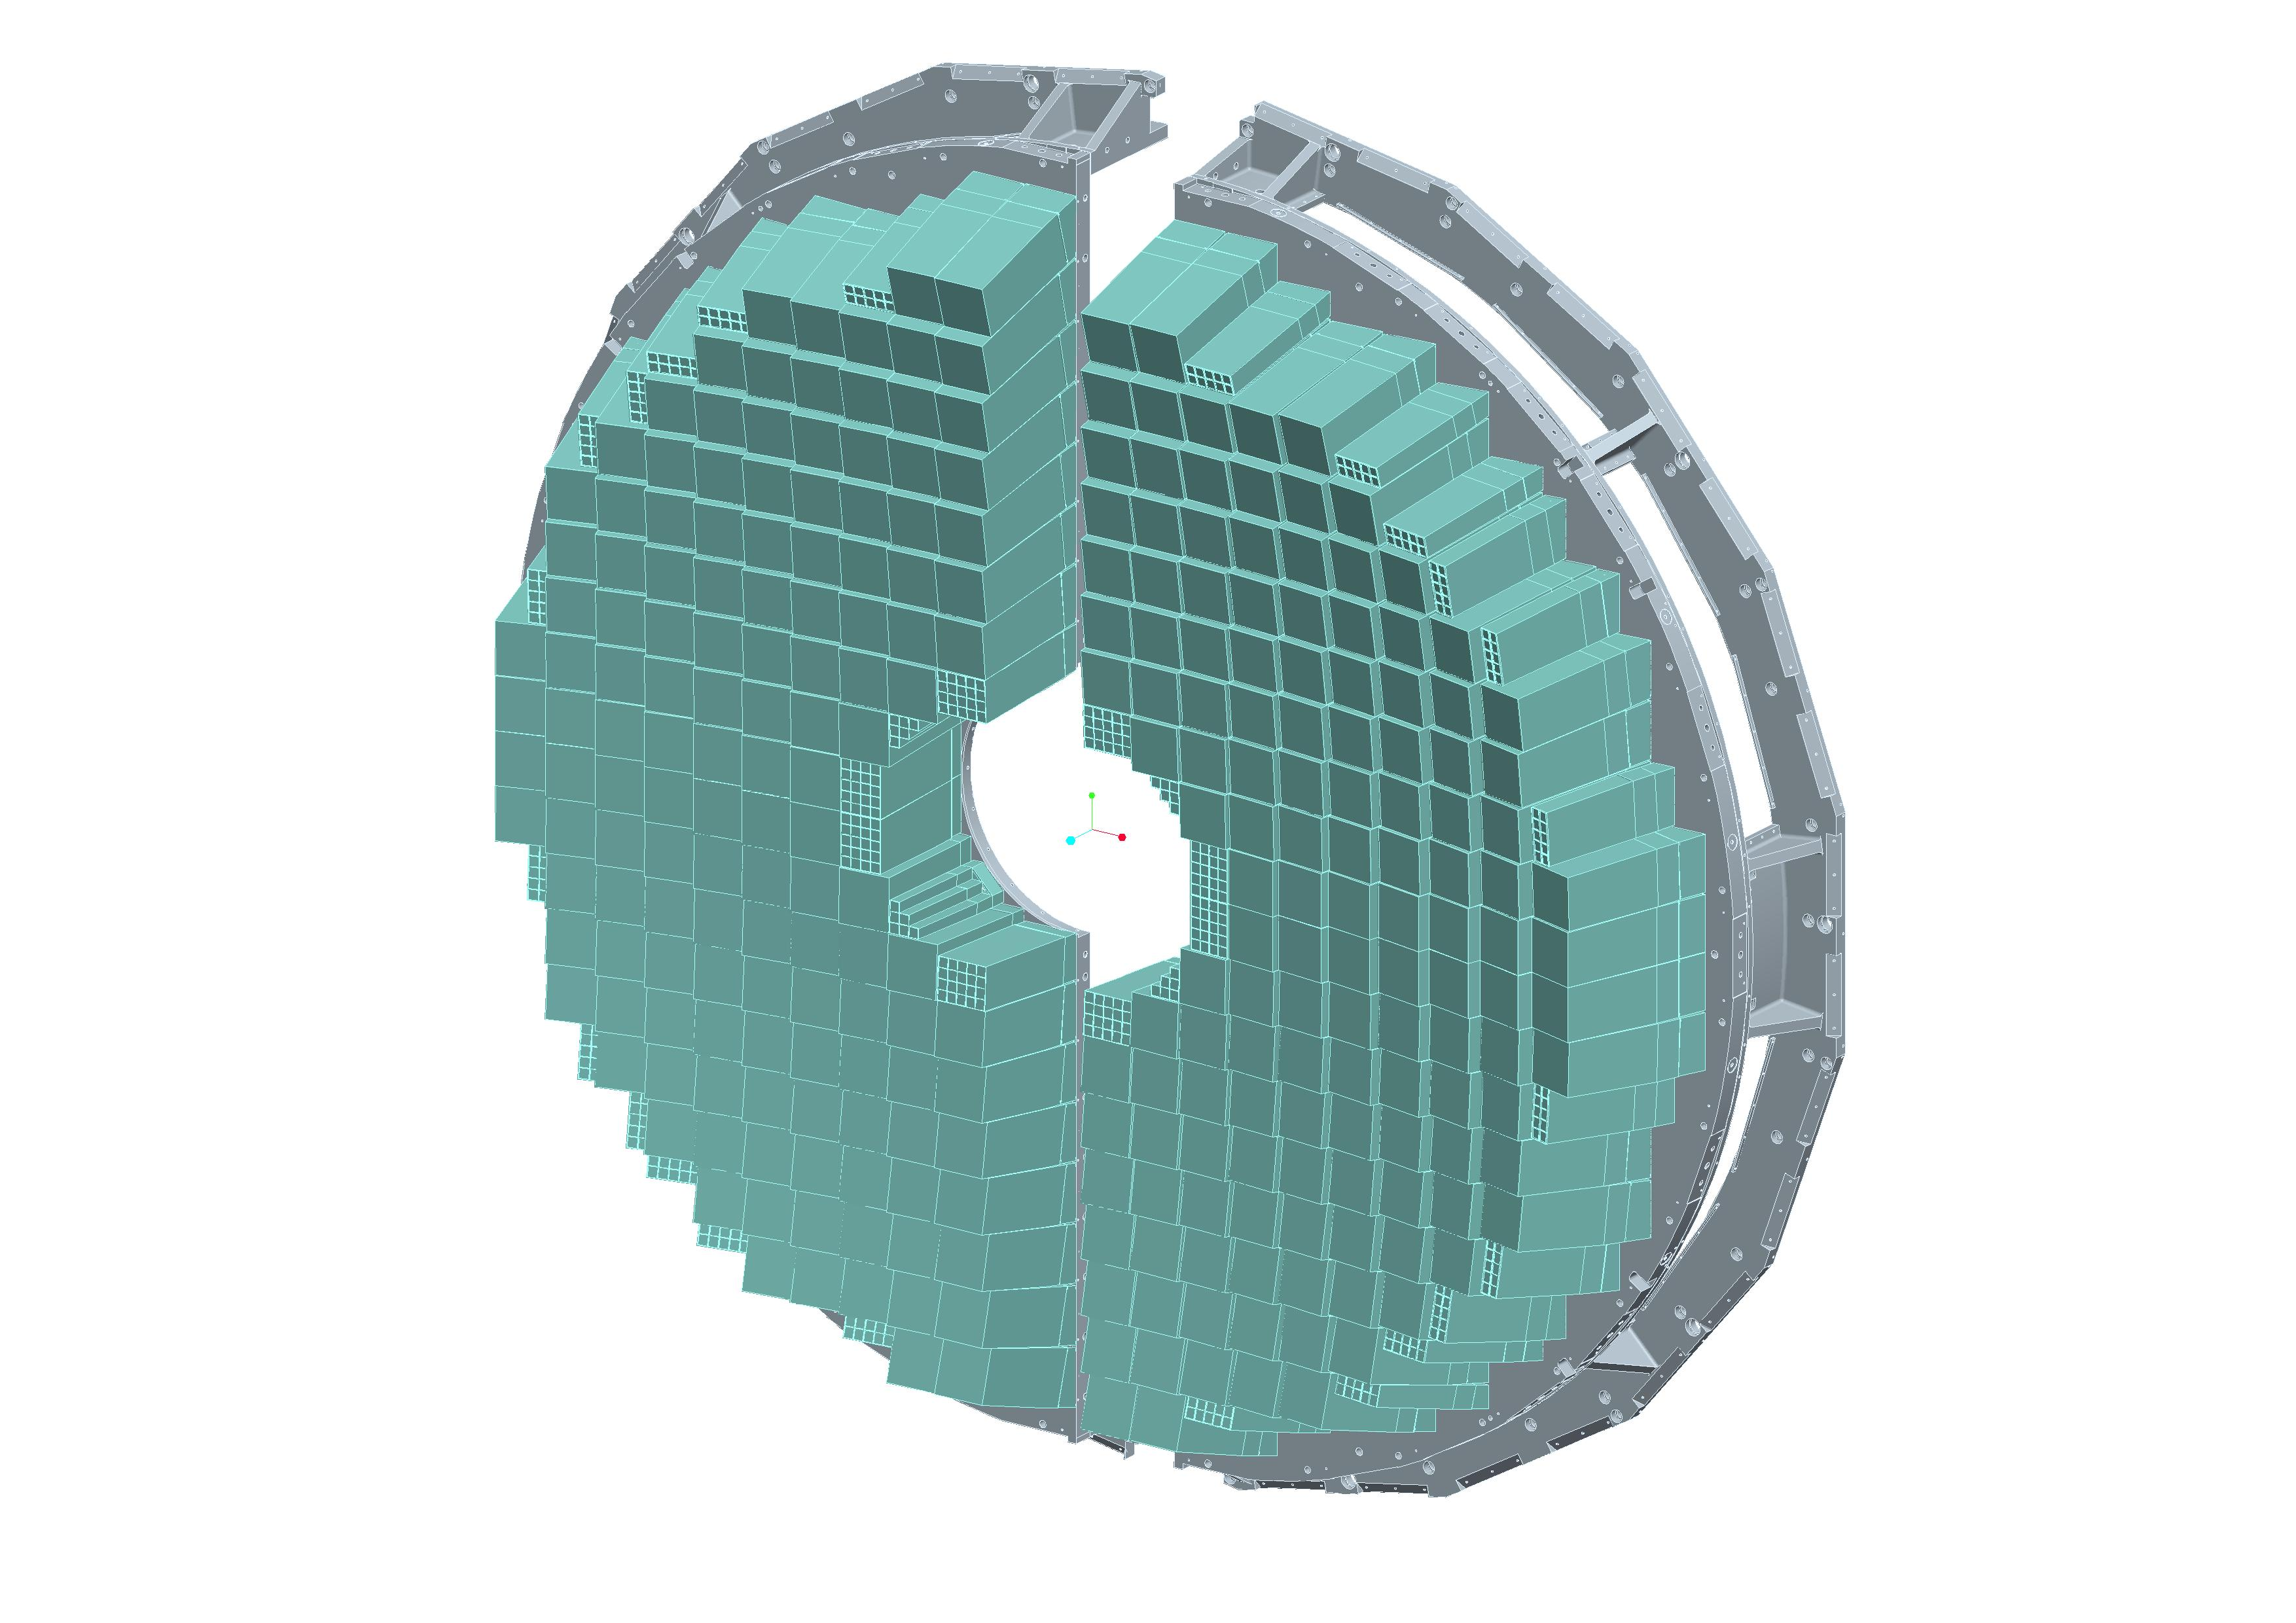
\includegraphics[scale=0.06]{THESISPLOTS/endcap_CMS.png}} 
\captionof{figure}{Top: Crystal mean time distribution for crystals in readout electronics EB$\pm$8. Crystal time is obtained from Laser data.
Bottom: Distribution of CCU timing shift in readout electronics due to hardware intervention  for EB~(top) and EE~(bottom). The adjustment for global timing shift per FED due to difference in light source for each CCU can be seen to reduce the possibility of CCU showing false timing shift. The figures show the distributions of the $\Delta t_{CCU} $ with corresponding RMS values before~(left) and after~(right) the global shift has been subtracted. }
\label{fig:TimeLaser}
\end{center}

Using the average subtraction method with the laser data, we can measure each CCU timing shift to within 0.2~(0.5)~ ns in EB~(EE) precision. This tool and procedure allow for adjusting the hardware timing settings at CMS data taking site in Point5 at Cessy, France. However some validation studies for the reliance and efficiency of this tool is yet to be performed.  

%%%%%%%%%%%%%%%%%%%%%%%%%%%%%%%%%%%%%%%%%%%%%%%%%%%%%%%%%%%%%%%%%%
\subsubsection{Timing Bias}
%%%%%%%%%%%%%%%%%%%%%%%%%%%%%%%%%%%%%%%%%%%%%%%%%%%%%%%%%%%%%%%%%%
The  Ratio algorithm described in previous sections for extracting the amplitude and time of an event from the ten digitized samples for a given crystal or channel is assumed to performed smoothly for all energies of a given initial particle impinging on the crystal. However, during collision, this is not the case, especially during gain transition points of the MGPA. An inherent bias in the timing measurement is introduced for incoming electromagnetic particles with energy above the gain transition point. The energy in GeV units deposited by an incoming particle on each crystal, $i$ is given by the signal amplitude $A_{i}$, in ADC counts and other correction and conversion factors using the equation:
\begin{equation}
    E_{i} =  G \cdot S_{i}(t) \cdot C_{i} \cdot A_{i} 
\end{equation}
where $G$ is an ADC-to-GeV factor with value equal to 0.039~(0.063) in EB~(EE). $C_{i}$ is the inter-calibration coefficients accounting for different channel response and $S_{i}(t)$ is correction term (usually from laser data) accounting for radiation-induced channel response  and changes as a function of time. The Gain 1 transition point occurs at 4096 ADC counts corresponding to 159.744~GeV in EB and 258.048~GeV in EE. The subsequent Gain 6 and 12 transitions are at energy values of TeV range.
The bias in timing introduced as a result of these gain transitions cannot be corrected at hardware  or calibrated away rather we developed a method of applying these timing bias corrections at the standard CMS Software~(CMSSW) reconstruction package.
Using reconstructed hits with same selection as offline timing calibration, selected hits are also required to be path of a basic cluster~(usually $9\times 9 $ or $25\times 25$ matrix of crystals) to ensure that they are electromagnetic objects produced from proton-proton collisions. These hits must have amplitude with channel noise consideration above 10 ADC counts, in order to reject hits with very large timing biased and must be overcome the swiss-cross variable selection threshold. A distribution of the hit time against its amplitude is plotted and then sliced in bins of amplitude. Each bin with having at least 7 hits is fitted using a Gaussian function constrained within $\pm 7$~ns. The average or mean and standard deviation or RMS of this distribution is extracted and plotted again its corresponding amplitude or energy bin content to give a distribution of mean against amplitude and standard deviation or resolution against amplitude. This procedure is performed for different Modules or pseudo-rapidity~($\eta$) ranges starting from $\eta = 0$ which is Module1 in barrel to $\eta = 3$ for high-eta in endcap.
Figure \ref{fig:TimeBias} shows these distribution for different CMSSW release~(CMSSW44X) where the these bias corrections have not been applied to the software release~(CMSSW5XY) in reconstruction where they have been applied. The dataset used for this reconstruction is the \textit{DoubleElectron} and \textit{Photon} dataset processed using CMSSW44X release during LHC RUN 1 and later reprocessed using CMSSW53X with the bias corrections we developed applied. All CMSSW releases beyond CMSSW5XY now have these bias corrections applied. 

\begin{center}\label{TimeBias}
\centering
\mbox{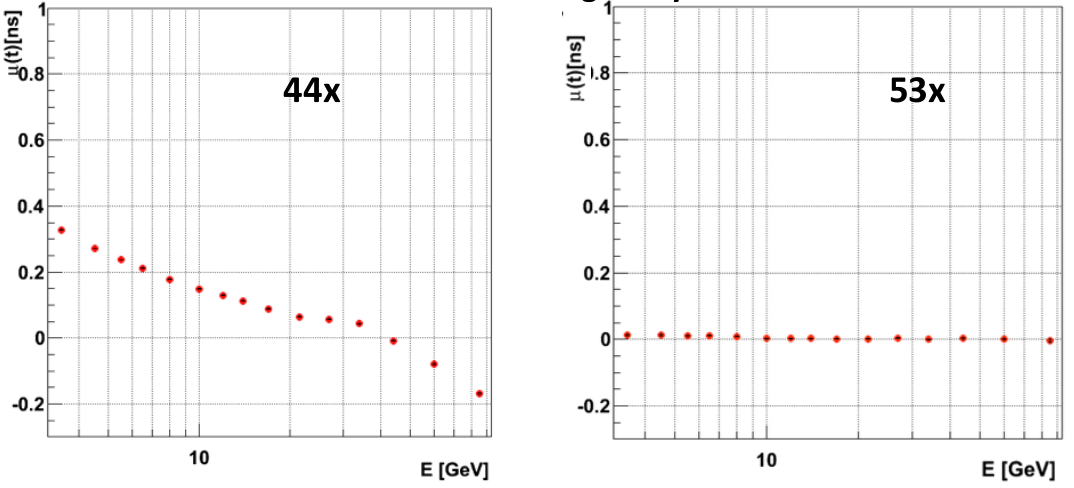
\includegraphics[scale=0.45]{THESISPLOTS/AmplitudeVsTimeCMSSW_Comparison.png}}
%\mbox{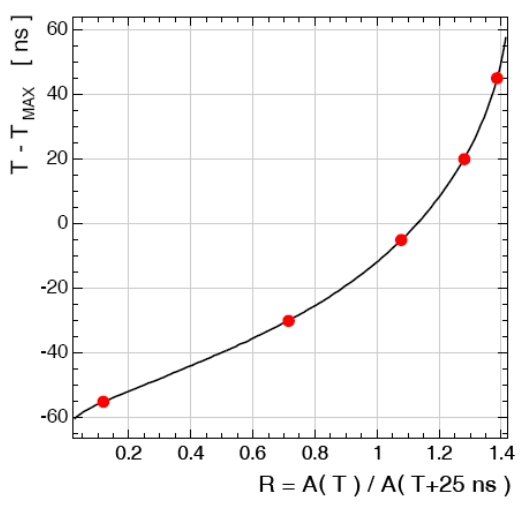
\includegraphics[scale=0.45]{THESISPLOTS/TMaxPhaseVsRatio.png}}
%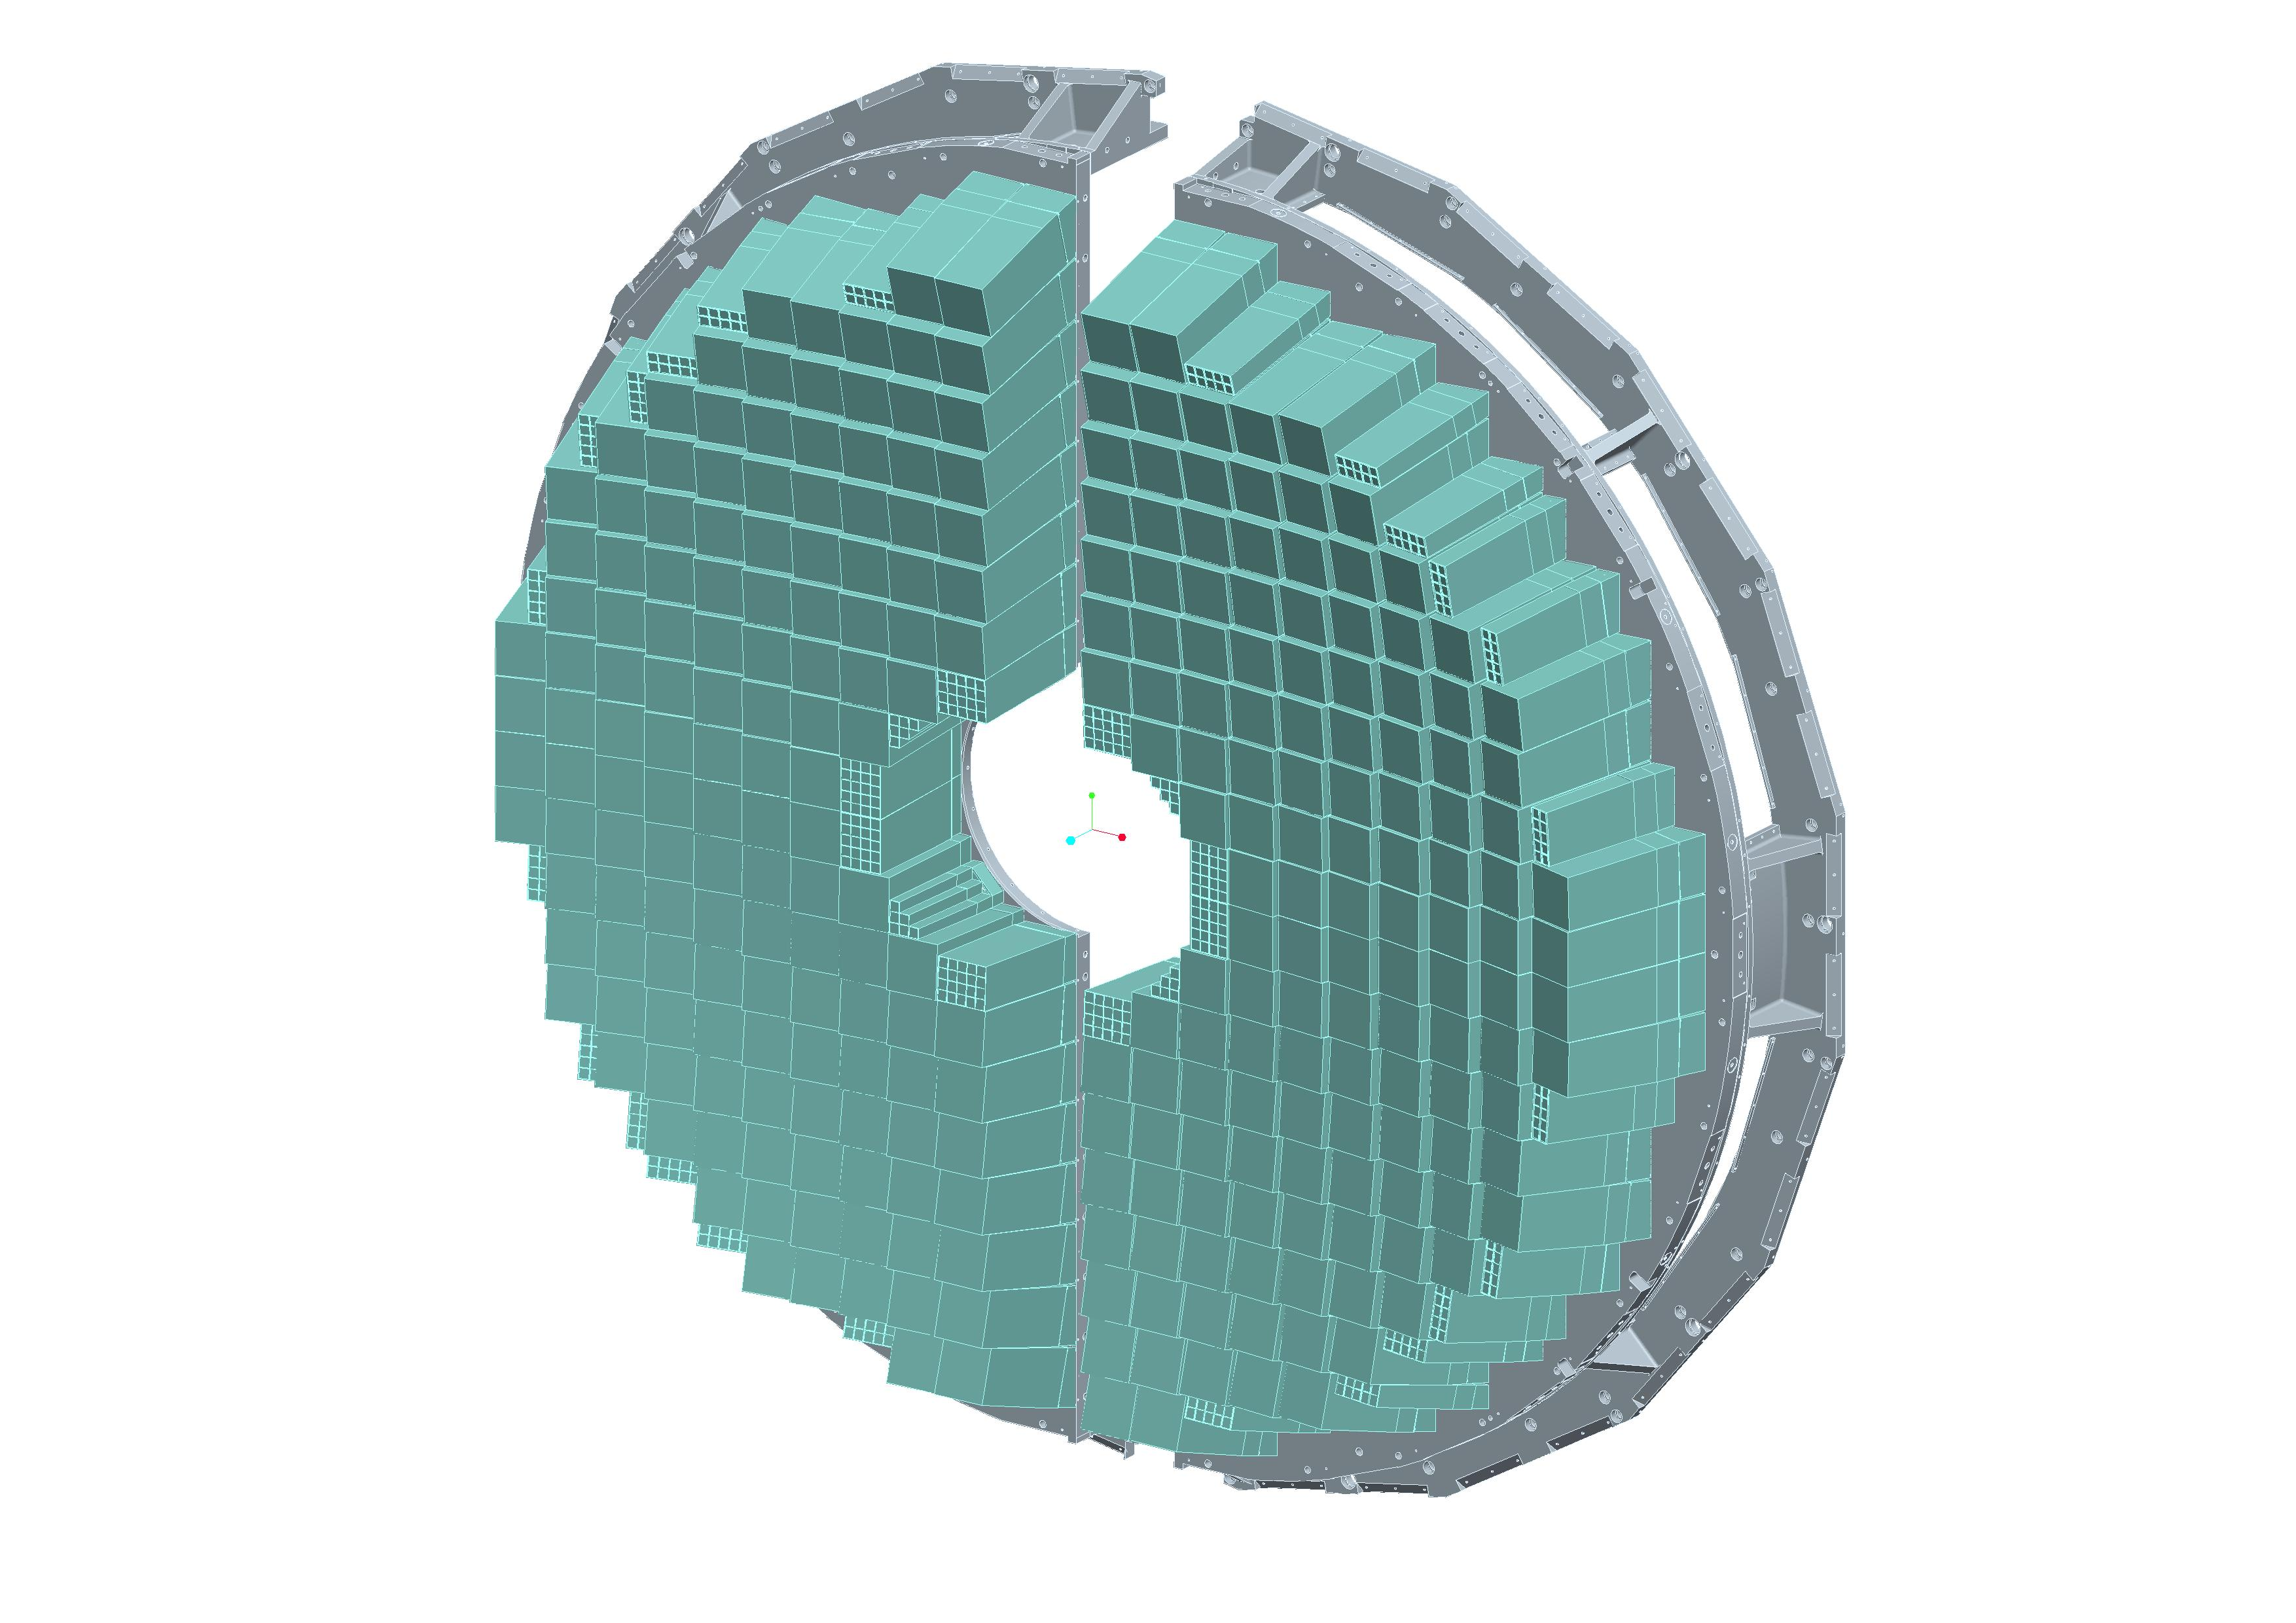
\includegraphics[scale=0.06]{THESISPLOTS/endcap_CMS.png}} 
\vspace{4cm}
\mbox{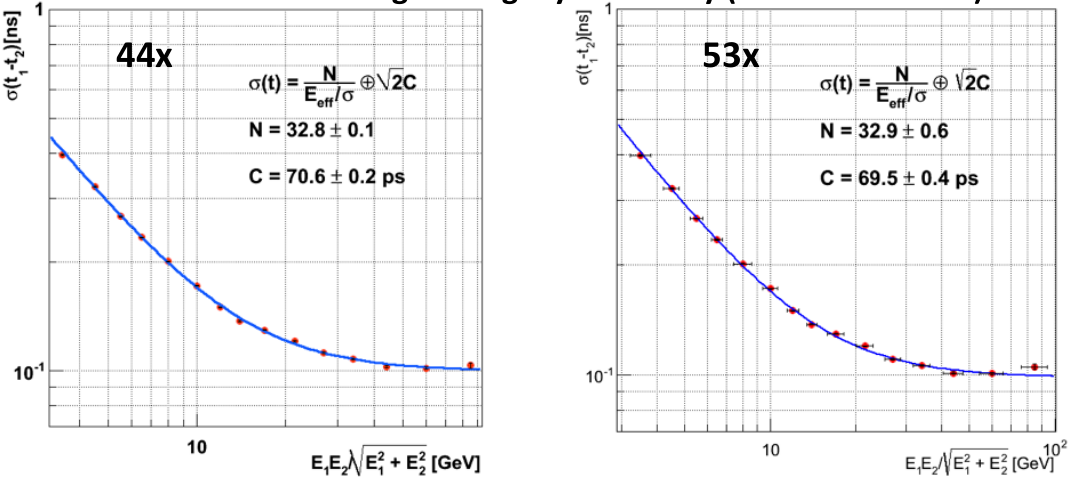
\includegraphics[scale=0.46]{THESISPLOTS/TimingResolutionCMSSW_Comparison.png}}
%\mbox{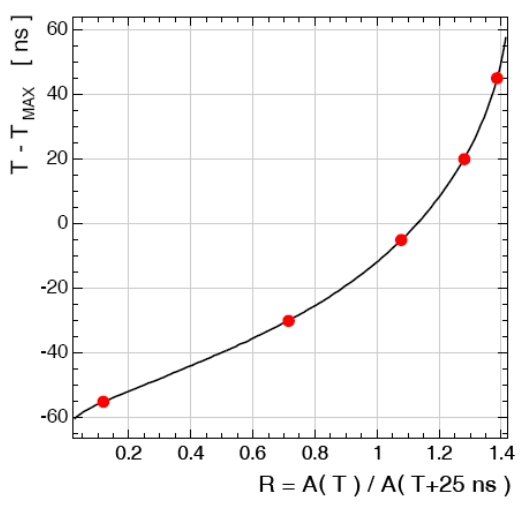
\includegraphics[scale=0.45]{THESISPLOTS/TMaxPhaseVsRatio.png}}
%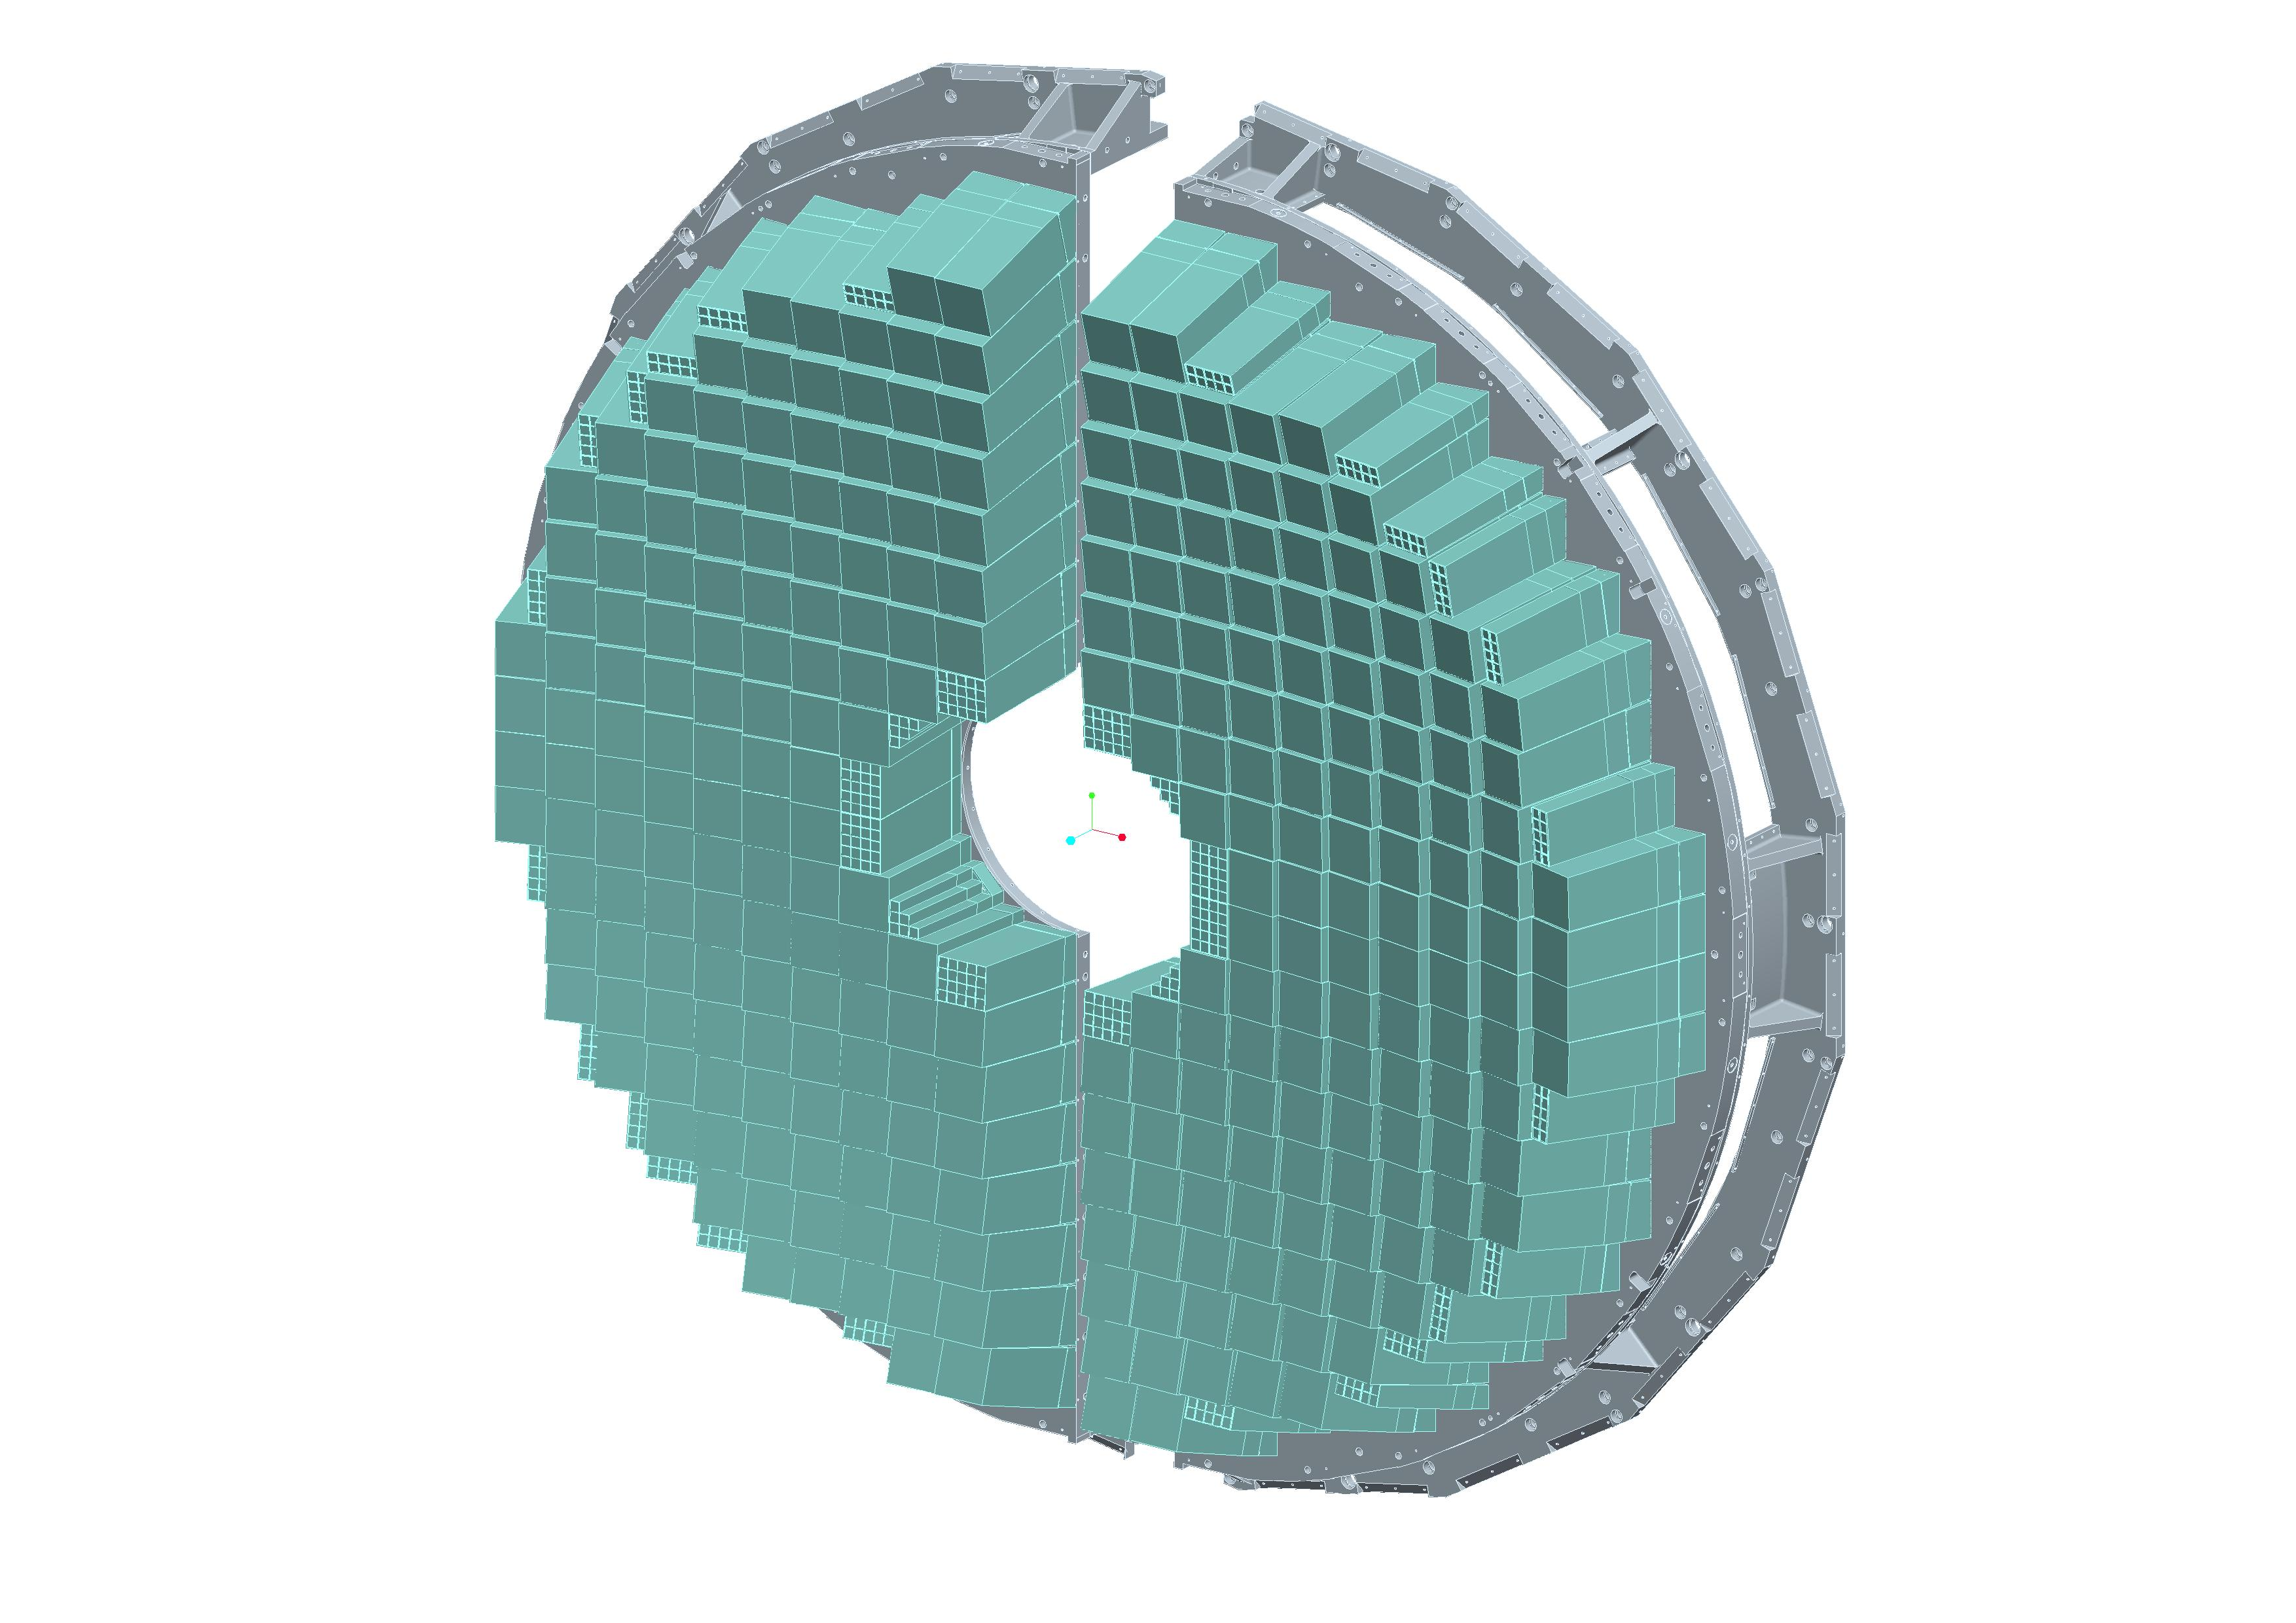
\includegraphics[scale=0.06]{THESISPLOTS/endcap_CMS.png}} 
\captionof{figure}{Top: Distribution of mean time as a function of crystal energy for EB prior~(left) and after~(right) timing bias corrections depending on amplitude developed have been applied.\newline
Bottom: Distribution of timing resolution as a function of crystal energy for EB prior~(left) and after~(right) timing bias corrections depending on amplitude developed have been applied.}
\label{fig:TimeBias}
\end{center}

Figure \ref{fig:EtaDep} show the distribution of the mean and standard deviation for different modules in barrel and sections in endcap. The timing resolution do not show any dependence on pseudo-rapidity~($\eta$), however minor dependence on event run number and different electronics or trigger towers have been observed. These small effects are yet to be understood and provides a challenge in realising using proton-proton collision data, ECAL timing resolution as initially observed during tests using electron beams.

\begin{center}\label{EtaDep}
\centering
\mbox{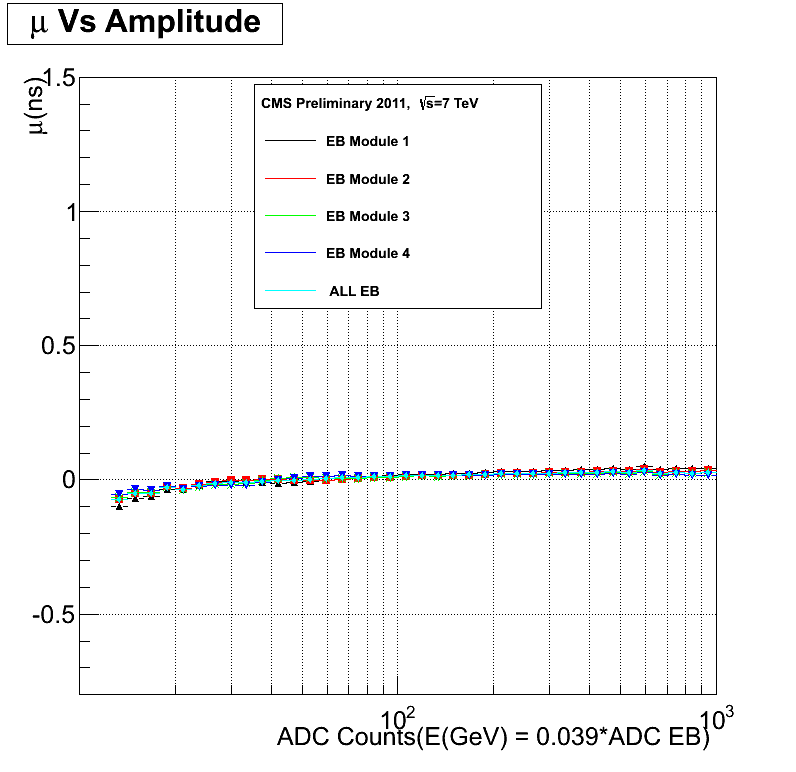
\includegraphics[scale=0.25]{THESISPLOTS/EB_TimeVsAmplitude_StabilityCMSSW_5_3_X.png} \quad
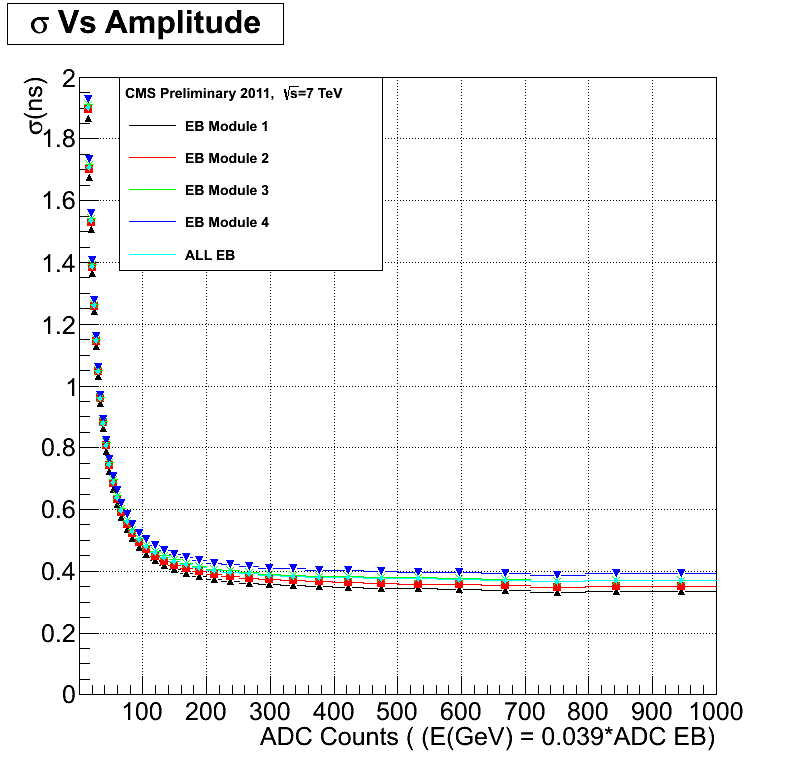
\includegraphics[scale=0.25]{THESISPLOTS/EB_SigmaVsAmplitude_Stability_In_CMSSW_53X.png}}
%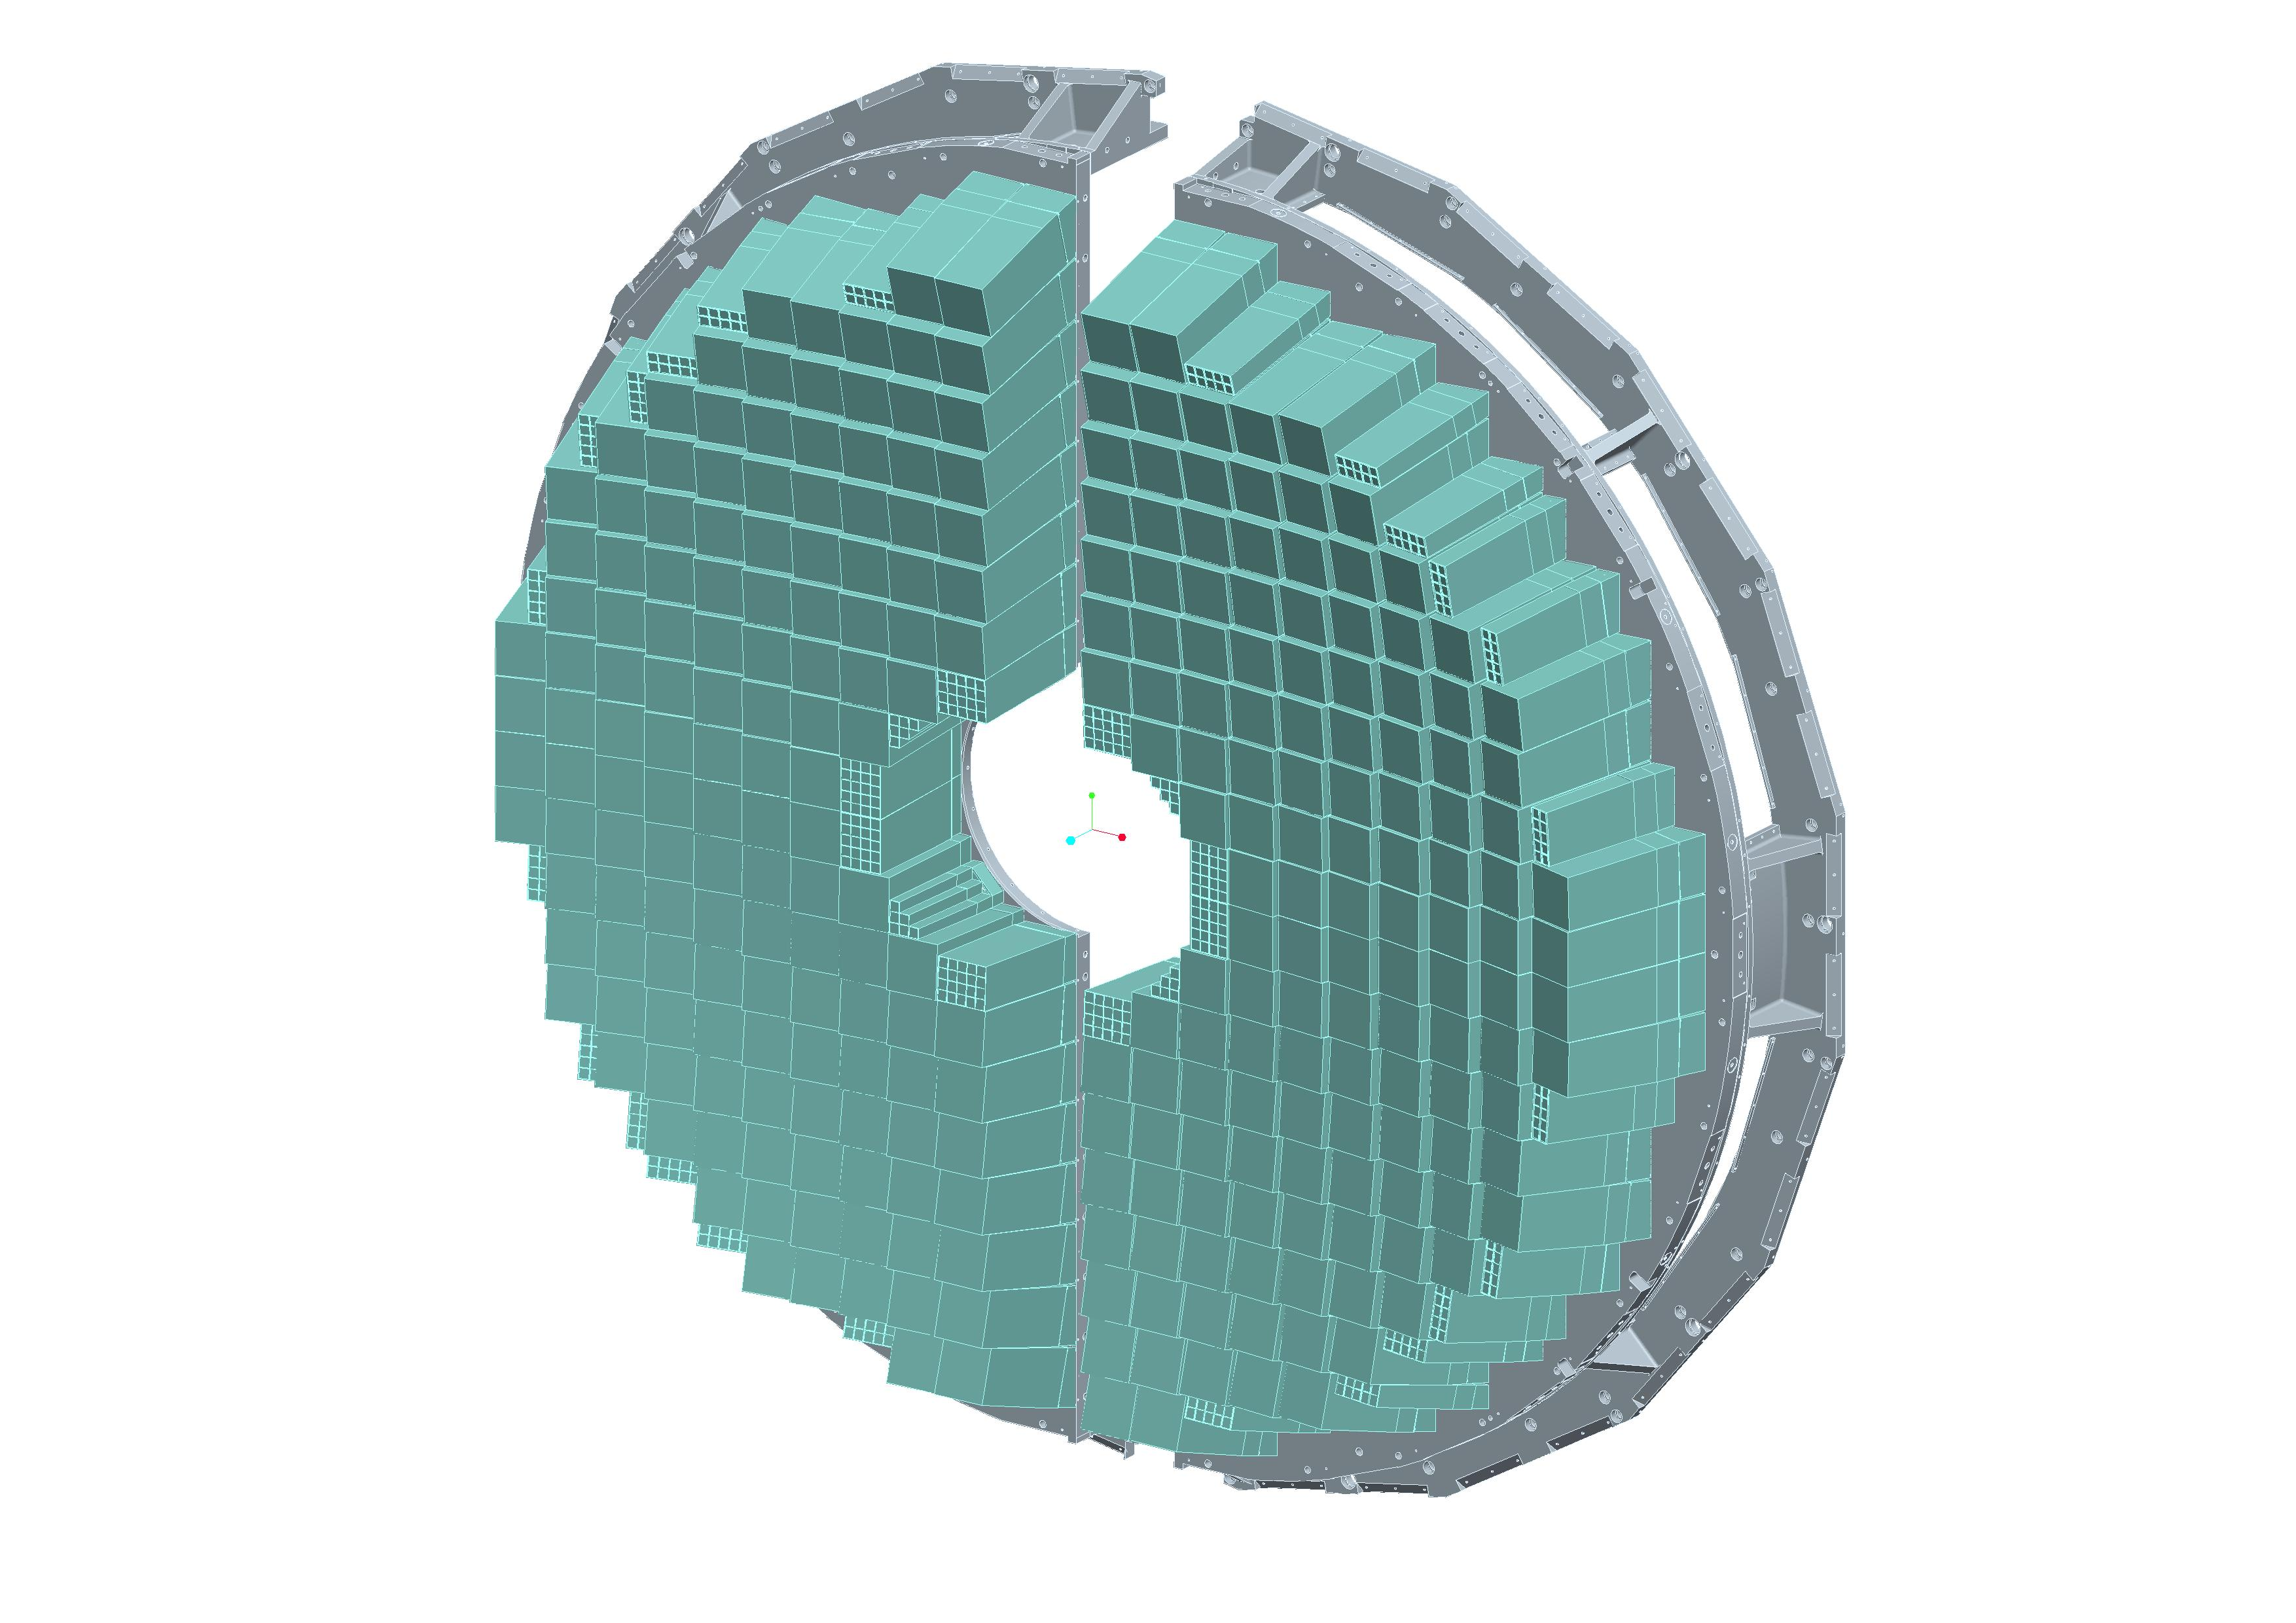
\includegraphics[scale=0.06]{THESISPLOTS/endcap_CMS.png}} 
\vspace{0.5cm}
\mbox{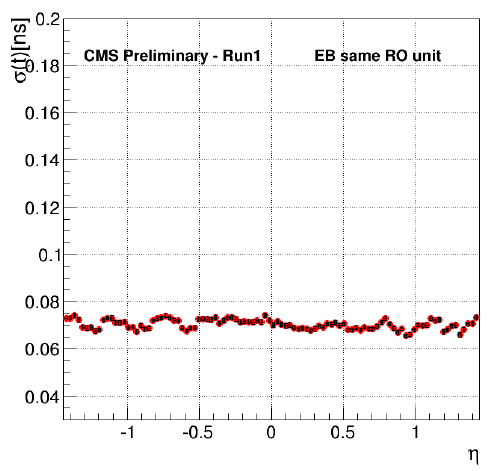
\includegraphics[scale=0.6]{THESISPLOTS/TimeResolution_Vs_Eta.png}}
%\mbox{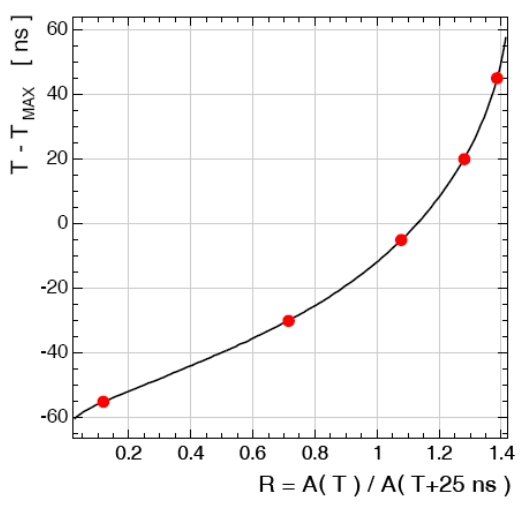
\includegraphics[scale=0.45]{THESISPLOTS/TMaxPhaseVsRatio.png}}
%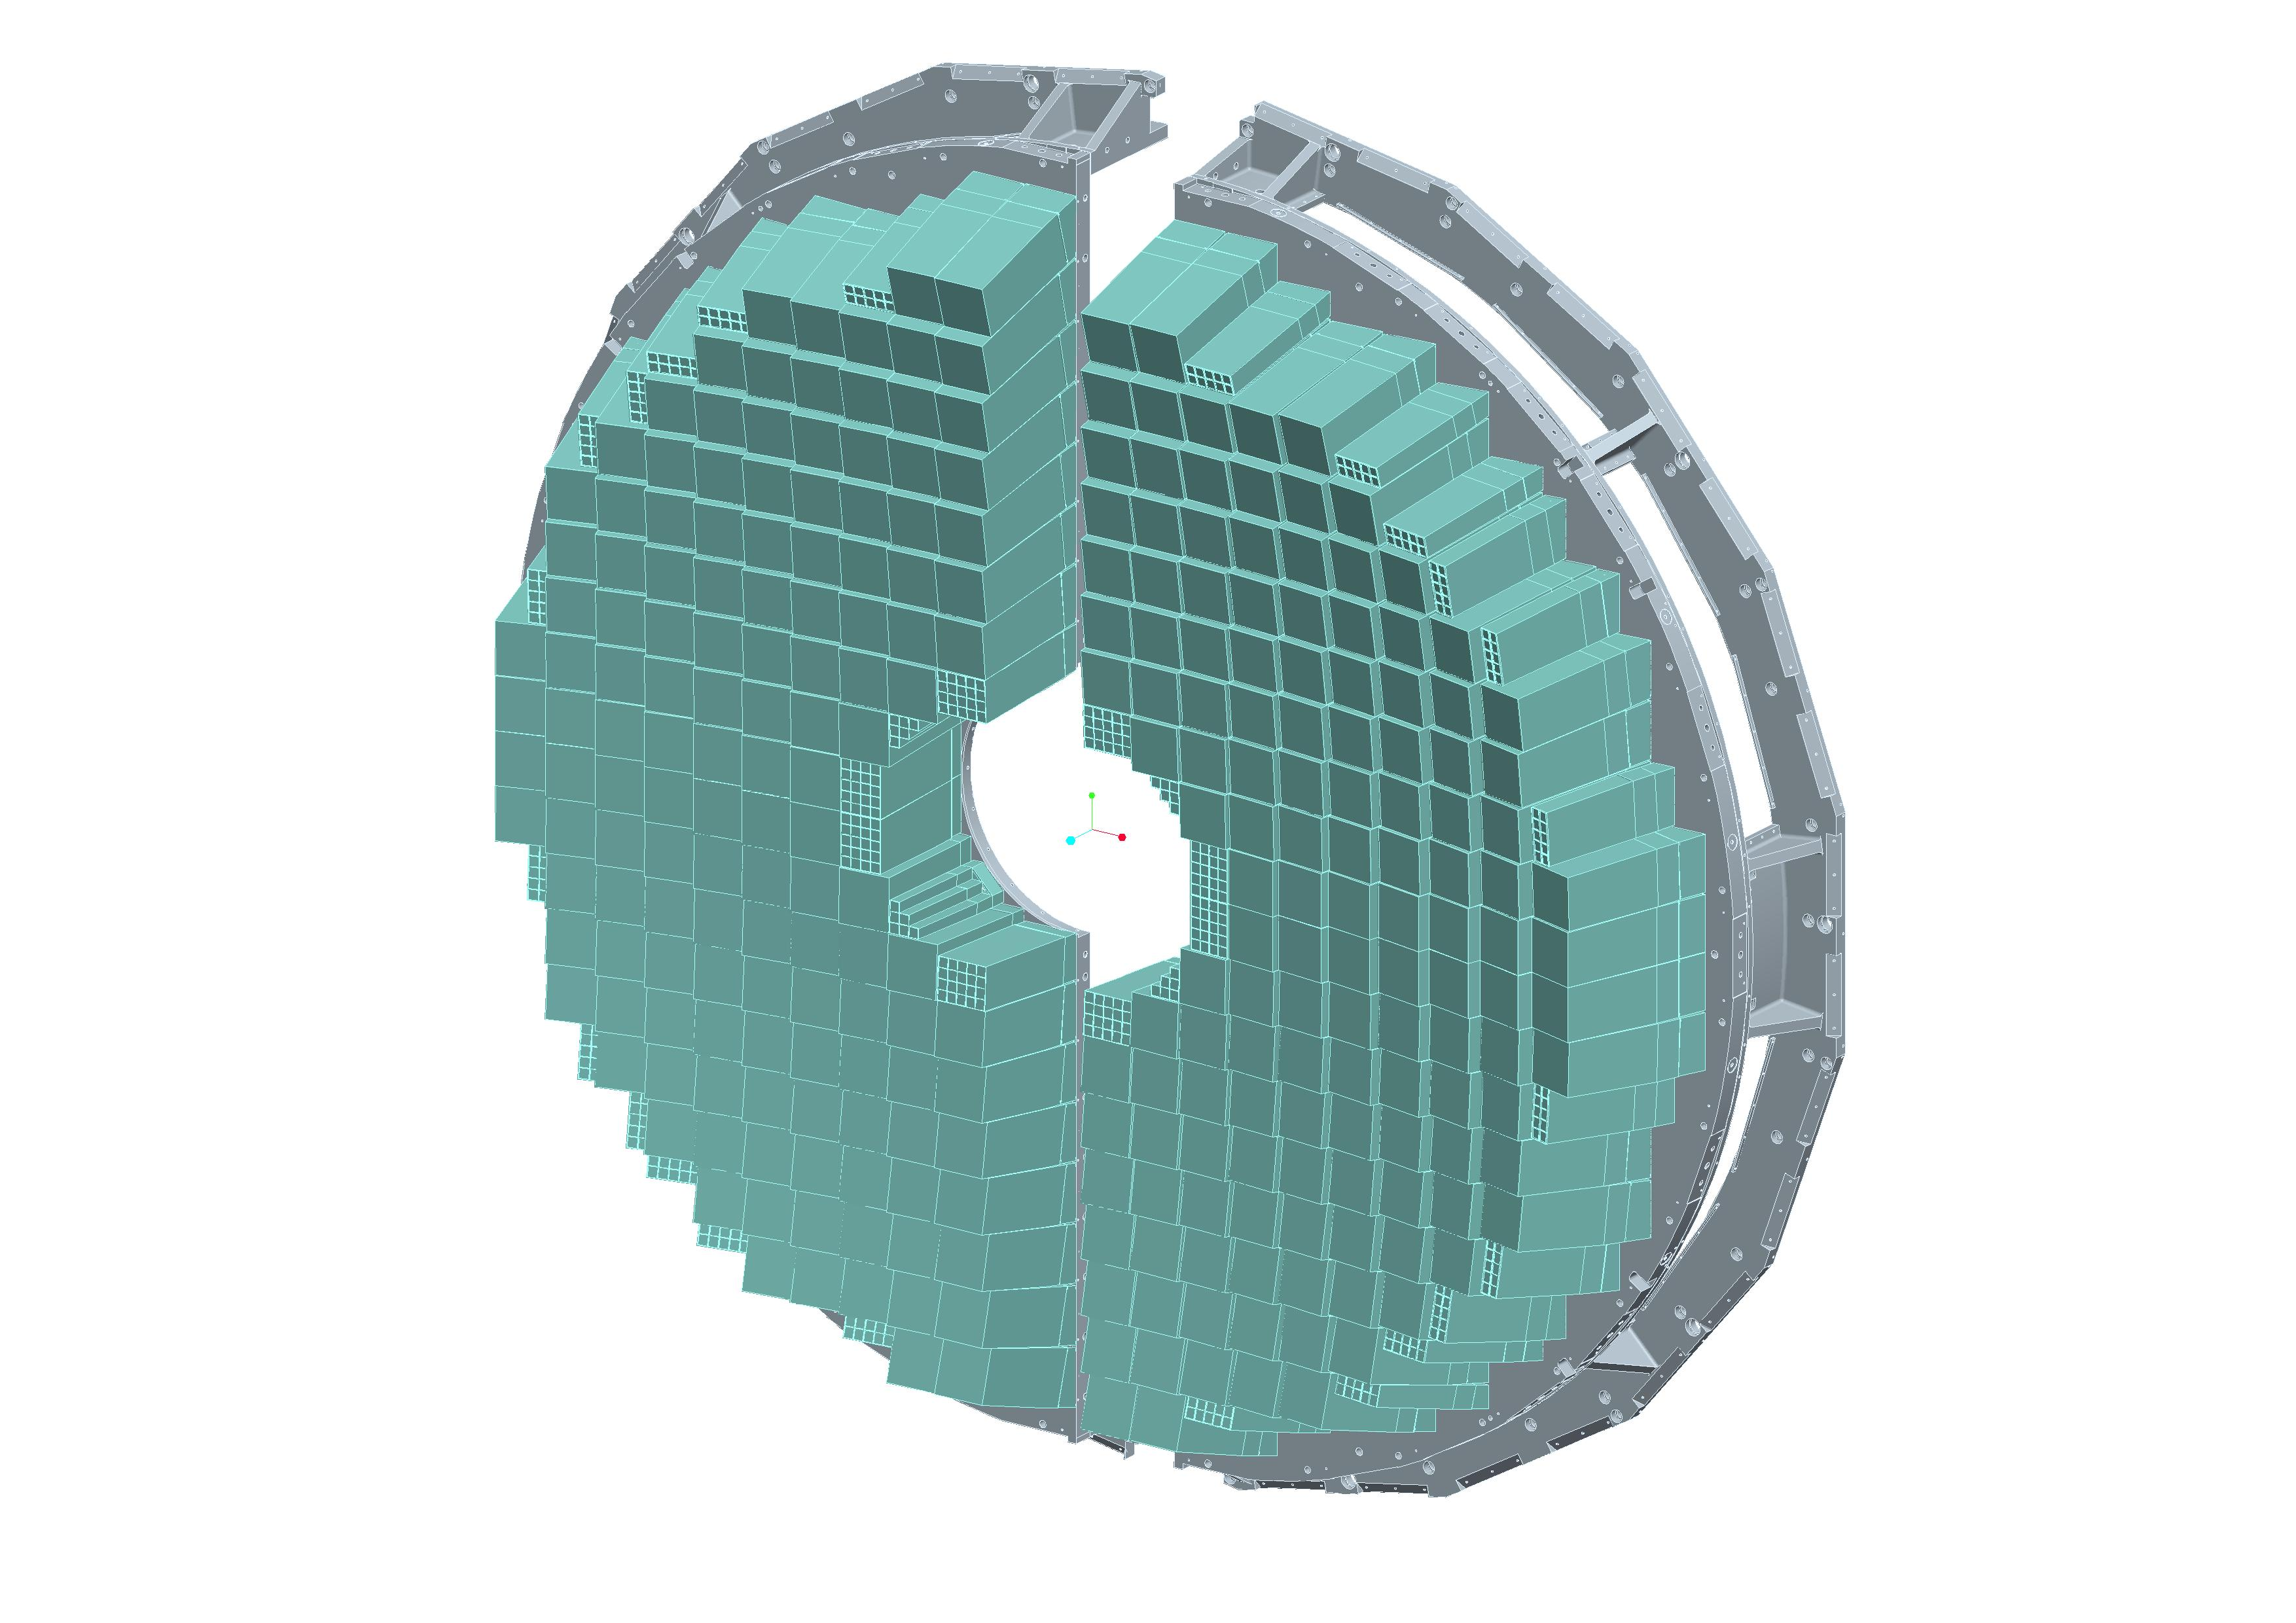
\includegraphics[scale=0.06]{THESISPLOTS/endcap_CMS.png}} 
\captionof{figure}{Top: Distribution of mean time as a function of amplitude~(left) and Resolution as a function of amplitude~(right) for different pseudo-rapidity regions in the barrel. \newline
Bottom: All modules in EB combined timing resolution as a function against $\eta$ crystals in the same readout electronics in  barrel~(EB). }
\label{fig:EtaDep}
\end{center}

%%%%%%%%%%%%%%%%%%%%%%%%%%%%%%%%%%%%%%%%%%%%%%%%%%%%%%%%%%%%%%%%%%
%%%%%%%%%%%%%%%%%%%%%%%%%%%%%%%%%%%%%%%%%%%%%%%%%%%%%%%%%%%%%%%%%%
\subsection{Electromagnetic Calorimeter Timing Performance}
%%%%%%%%%%%%%%%%%%%%%%%%%%%%%%%%%%%%%%%%%%%%%%%%%%%%%%%%%%%%%%%%%%
Timing calibration has been performed to properly align the timing of an incoming event which might be effected due to variations of event time in different runs, poor inter-calibrations especially between different front end electronics, biased on timing due to timing dependence on energy, reduction in \pb crystal transparency due to radiation, hardware intervention during machine repairs and other yet understood causes. To ensure that the calibration procedure has improved on the timing alignment, we study the timing performance of the ECAL crystals and validate this studies using events electrons produced from the decay of a $\PZ$ boson  i.e $\PZ \rightarrow \Pelectron \Ppositron$.  The decay of a $\PZ$ boson is a very well understood signal and with effects due to poor event reconstruction or detector effects very well understood and measured. 
\newline
The main idea is to use these two electrons or any two reconstructed candidate "objects" which in principle should have the same ECAL crystal arrival time and then use their measured time difference as a measure of timing resolution of the \pb crystals in ECAL. These two reconstructed candidate objects can be:
\begin{enumerate}
\item Two crystals within the same electron super cluster.
\item Neighbouring crystals with a particular supercluster and sharing the same supercluster energy. This has the advantage of minimizing shower propagation effects.
\item Two crystals each from the different electron superclusters.
\item Or the two well reconstructed and energy corrected superclusters from the $\PZ$ decay. 
\end{enumerate}

In using reconstructed electron, we considered following additional contributions to the electron time:
\begin{enumerate}
\item The bending of the electron path due to the presence of the 3.8~T magnetic field of the CMS detector.
\item  Displaced collisions because "partons"~(subparticles) in the protons of the proton-proton~(p-p) bunches did not collide at exactly the collision point or nominal interaction point~(IP).
\item The collision developed over the full duration of the overlap of the proton bunches. This is known as the spread in collision timing and account for about 183~ps in worsening of timing resolution.
\end{enumerate}

The Time-Of-Flight~(TOF) of the electron from the I produced in a nominal collision is assumed to be zero on average in the time calibration algorithm since the electrons or photons travel with speed very close to on even the speed of light. However, there are slight variations due to the difference in originated point or vertex position of these electrons or photons. In the case of electrons, the true vertex position of the electron can be reconstructed and the small TOF variations corrected for, but in the case of photons, since photons do not leave in track signals in the tracker detector, it is a bit challenging to account for these variations in TOF due to no knowing the true primary vertex where the photon originated from. There are active studies ongoing to be able to use ECAL timing to reconstruct the true primary vertex of a photon using the information of its arrival time in the ECAL, cluster position and energy. This kind of studies is motivated by the Higgs decay into two photon process  i.e $H \rightarrow \gamma \gamma $, as we continue towards understanding the properties of the recently observed scalar boson particle decay into to photon process.  

Thus photons are used for timing calibration of the \pb crystals while electrons or electron candidates in general are used for studying the timing performance.
Figure \ref{fig:ZeeTimePerformance}, shows the timing resolution obtained  by extracting the timing of the seed crystal~(crystal with highest energy) within the electron suspercluster (a) and the time difference of both electrons with the corrections due to time of flight applied (b). Without contribution from the fact that proton collisions develops across the entire beam luminous region of nearly 5.5~cm referred to as proton collision time ~(corresponding to about $\sigma(t_{colision}) = \sigma(t_{Z}) = 183~ps$) removed in quadrature gives 232~ps in EB and 384~ps in EE timing measurements from $\PZ$ events. This is pretty good resolution for detecting late electromagnetic particles if produced during a new kind of particle interaction non in the SM.
The electrons used are required to isolated to differentiate them from hadrons by using simple cluster shape  selection requirements. Each electron candidate making the $\PZ$ must have  a transverse energy bigger than 10~GeV. Both electrons must also have their invariant mass bounded from below~(above) by a 60(150)~GeV cut i.e $ 60~GeV < m_{inv}(e_{1},e_{2}) < 150~ GeV$ to make a good $\PZ$ boson candidate. 

\begin{center}\label{TimeRES}
\centering
\mbox{
\includegraphics[width=3in]{/home/tensr/Documents/ECAL_NOTES/PLOTS/2013/ECALTDRPLOTS/EB-EB-Time-of-seed.png}\quad
\includegraphics[width=3in]{/home/tensr/Documents/ECAL_NOTES/PLOTS/2013/ECALTDRPLOTS/EE-EE-Time-of-Seed.png}}
\captionof{figure}{Ecal absolute time of a single reconstructed electron in $\PZ \rightarrow \Pelectron \Ppositron$ decay. The electron time is the seed~(crystal with highest energy deposit)time of the electron.(a) in in EB and (b) in EE} 
\label{fig:ZeeTimePerformance}
\end{center}

\begin{center}
%\begin{figure}
\centering
\mbox{
\includegraphics[width=3in]{/home/tensr/Documents/ECAL_NOTES/PLOTS/2013/ECALTDRPLOTS/EB-EB-TOF-Corr-difference-of-seed.png}\quad
\includegraphics[width=3in]{/home/tensr/Documents/ECAL_NOTES/PLOTS/2013/ECALTDRPLOTS/EE-EE-TOF-Corr-difference-of-seed.png}}
\captionof{figure}{Ecal time difference between the two reconstructed electrons in $\PZ \rightarrow \Pelectron \Ppositron$ decay. The electron time is the seed~(crystal with highest energy deposit) time with additional correction due to the time of flight of the electron.(a) in in EB and (b) in EE} 
\label{fig:ZeeTimePerformance}
%\end{figure}
\end{center}
To compare the timing resolution obtain during test beam studies to that obtained recently at the end of LHC Run 1, a similar figure is made as shown in figure \ref{fig:ZeeTimeResolution} produced from the $\PZ \rightarrow \Pelectron \Ppositron$ decay events with the timing difference between the two electrons plotted as a function of the effective amplitude normalised to the noise in the ECAL Barrel for 2011 and 2012 data. The noise term in consistent with results obtained during test beam while the constant term is bout 150~ps much larger than that obtained from test beam studies. Its has been shown that effects such as poor inter-calibration between two different front end electrons, run dependence and radiation might be the reason for the  large constant term. There is active research ongoing towards archiving the test beam results, however the current value is good enough to use the ECAL timing as a variable to search for long-lived particles.
\begin{center}\label{ECALTRes}
%\begin{figure}
\centering
\mbox{
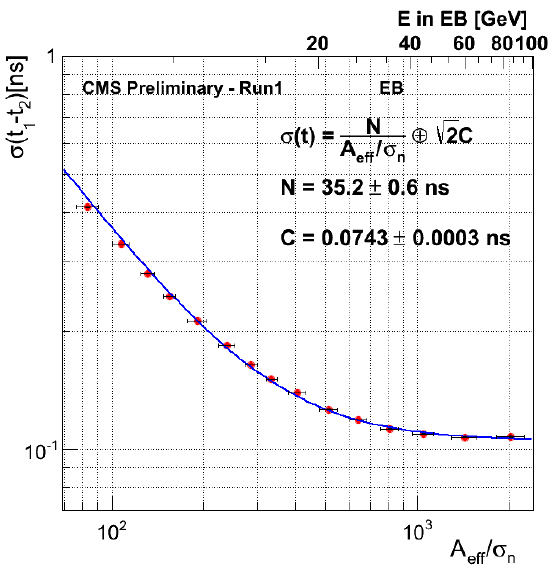
\includegraphics[scale=0.5]{THESISPLOTS/NeigboMethodECALTimeRes.png}\quad
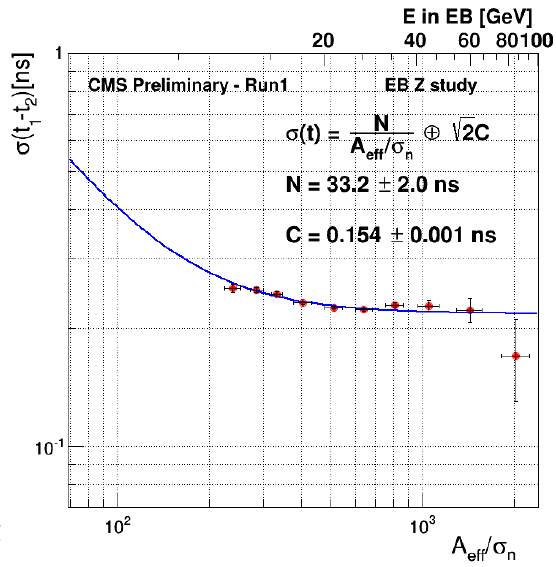
\includegraphics[scale=0.5]{THESISPLOTS/ZeeECALTimeRes.png}}
\captionof{figure}{Resolution of time difference between two most energetic crystals in the same readout unit of an ECAL cluster as a function of effective amplitude- The Neighbouring crystal method(left),  Resolution of time difference between the two reconstructed electrons in $\PZ \rightarrow \Pelectron \Ppositron$ decay as a function of  effective amplitude($A_{eff} = A_{1}A_{2}/\sqrt{A^{2}_{1} + A^{2}_{2}}$), for both electrons in EB; The $\PZ$ method~(right).
The noise  term $N$ is the same as test beam for bother methods while the constant term $\bar{C}$ is better for the Neighbouring crystal method~(70~ps)  than for the $\PZ$ method ~(150~ps) indicating the effect due to different intercalibrations between two different readout of front end electronics.} \label{fig:ZeeTimeResolution}
%\end{figure}
\end{center}
Table \ref{tab:TIMERes} shows Ecal timing resolution for 2011 and 2012 dataset. 

\begin{center}\label{CMSRES}
\centering
 %\setlength{\abovecaptionskip}{0pt}
  %\setlength{\belowcaptionskip}{10pt}
 % \topcaption{GMSB,GGM Phenomenology and Relevant final states}
  \begin{tabular}{cc|l|l} % p{0.1cm}|p{0.1cm}|}
  \hline \hline
 
 &  \multicolumn{1}{r}{\bfseries{ECAL Timing Resolution}} \\
  \hline \hline
&  \multicolumn{2}{c}{\bfseries{2011}} \\
   \hline
   & $\sigma_{eff}(t_{seed})$[ps]
        Absolute time
   & $\sigma_{eff}(t_{e1} - t_{e2})/\sqrt{2}$[ps]   Single Precision \\ \hline
   \textbf{EB} & 376  & 190 \\
      \textbf{EE} & 356  & 282 \\
      \hline \hline
& \multicolumn{2}{c}{\bfseries{2012}}  \\
   \hline
   & $\sigma_{eff}(t_{seed})$[ps]
        Absolute time
   & $\sigma_{eff}(t_{e1} - t_{e2})/\sqrt{2}$[ps]   Single Precision \\ \hline
   \textbf{EB} & 340  & 164 \\
      \textbf{EE} & 342  & 272 \\
      \hline \hline
 
  \end{tabular}
   \captionof{table}{Table Comparing Timing Resolution performance of 2011 with 2012}
 \label{tab:TIMERes} % for use in \ref{table1} if you want to refer to the table number
 \end{center}
%\end{table}

%\begin{center}
%\begin{tabular}{cc|c|c|c|c|l}
%\centering
%\cline{3-6}
%& & \multicolumn{4}{ c| }{Primes} \\ \cline{3-6}
%& & 2 & 3 & 5 & 7 \\ \cline{1-6}
%\multicolumn{1}{ |c| }{\multirow{2}{*}{Powers} } &
%\multicolumn{1}{ |c| }{504} & 3 & 2 & 0 & 1 &     \\ \cline{2-6}
%\multicolumn{1}{ |c  }{}                        &
%\multicolumn{1}{ |c| }{540} & 2 & 3 & 1 & 0 &     \\ \cline{1-6}
%\multicolumn{1}{ |c  }{\multirow{2}{*}{Powers} } &
%\multicolumn{1}{ |c| }{gcd} & 2 & 2 & 0 & 0 & min \\ \cline{2-6}
%\multicolumn{1}{ |c  }{}                        &
%\multicolumn{1}{ |c| }{lcm} & 3 & 3 & 1 & 1 & max \\ \cline{1-6}
%\end{tabular}
% \captionof{table}{Table Comparing Timing Resolution performance of 2011 Vs 2012}
% \label{tab:TIMERes} % for use in \ref{table1} if you want to refer to the table number
%\end{center}


%%%%%%%%%%%%%%%%%%%%%%%%%%%%%%%%%%%%%%%%%%%%%%
\label{ECAL Timing Calibration_chapter}
